% Options for packages loaded elsewhere
% Options for packages loaded elsewhere
\PassOptionsToPackage{unicode}{hyperref}
\PassOptionsToPackage{hyphens}{url}
\PassOptionsToPackage{dvipsnames,svgnames,x11names}{xcolor}
%
\documentclass[
]{article}
\usepackage{xcolor}
\usepackage{amsmath,amssymb}
\setcounter{secnumdepth}{5}
\usepackage{iftex}
\ifPDFTeX
  \usepackage[T1]{fontenc}
  \usepackage[utf8]{inputenc}
  \usepackage{textcomp} % provide euro and other symbols
\else % if luatex or xetex
  \usepackage{unicode-math} % this also loads fontspec
  \defaultfontfeatures{Scale=MatchLowercase}
  \defaultfontfeatures[\rmfamily]{Ligatures=TeX,Scale=1}
\fi
\usepackage{lmodern}
\ifPDFTeX\else
  % xetex/luatex font selection
  \setmainfont[]{Latin Modern Roman}
  \setmathfont[]{Latin Modern Math}
\fi
% Use upquote if available, for straight quotes in verbatim environments
\IfFileExists{upquote.sty}{\usepackage{upquote}}{}
\IfFileExists{microtype.sty}{% use microtype if available
  \usepackage[]{microtype}
  \UseMicrotypeSet[protrusion]{basicmath} % disable protrusion for tt fonts
}{}
\makeatletter
\@ifundefined{KOMAClassName}{% if non-KOMA class
  \IfFileExists{parskip.sty}{%
    \usepackage{parskip}
  }{% else
    \setlength{\parindent}{0pt}
    \setlength{\parskip}{6pt plus 2pt minus 1pt}}
}{% if KOMA class
  \KOMAoptions{parskip=half}}
\makeatother
% Make \paragraph and \subparagraph free-standing
\makeatletter
\ifx\paragraph\undefined\else
  \let\oldparagraph\paragraph
  \renewcommand{\paragraph}{
    \@ifstar
      \xxxParagraphStar
      \xxxParagraphNoStar
  }
  \newcommand{\xxxParagraphStar}[1]{\oldparagraph*{#1}\mbox{}}
  \newcommand{\xxxParagraphNoStar}[1]{\oldparagraph{#1}\mbox{}}
\fi
\ifx\subparagraph\undefined\else
  \let\oldsubparagraph\subparagraph
  \renewcommand{\subparagraph}{
    \@ifstar
      \xxxSubParagraphStar
      \xxxSubParagraphNoStar
  }
  \newcommand{\xxxSubParagraphStar}[1]{\oldsubparagraph*{#1}\mbox{}}
  \newcommand{\xxxSubParagraphNoStar}[1]{\oldsubparagraph{#1}\mbox{}}
\fi
\makeatother

\usepackage{color}
\usepackage{fancyvrb}
\newcommand{\VerbBar}{|}
\newcommand{\VERB}{\Verb[commandchars=\\\{\}]}
\DefineVerbatimEnvironment{Highlighting}{Verbatim}{commandchars=\\\{\}}
% Add ',fontsize=\small' for more characters per line
\usepackage{framed}
\definecolor{shadecolor}{RGB}{241,243,245}
\newenvironment{Shaded}{\begin{snugshade}}{\end{snugshade}}
\newcommand{\AlertTok}[1]{\textcolor[rgb]{0.68,0.00,0.00}{#1}}
\newcommand{\AnnotationTok}[1]{\textcolor[rgb]{0.37,0.37,0.37}{#1}}
\newcommand{\AttributeTok}[1]{\textcolor[rgb]{0.40,0.45,0.13}{#1}}
\newcommand{\BaseNTok}[1]{\textcolor[rgb]{0.68,0.00,0.00}{#1}}
\newcommand{\BuiltInTok}[1]{\textcolor[rgb]{0.00,0.23,0.31}{#1}}
\newcommand{\CharTok}[1]{\textcolor[rgb]{0.13,0.47,0.30}{#1}}
\newcommand{\CommentTok}[1]{\textcolor[rgb]{0.37,0.37,0.37}{#1}}
\newcommand{\CommentVarTok}[1]{\textcolor[rgb]{0.37,0.37,0.37}{\textit{#1}}}
\newcommand{\ConstantTok}[1]{\textcolor[rgb]{0.56,0.35,0.01}{#1}}
\newcommand{\ControlFlowTok}[1]{\textcolor[rgb]{0.00,0.23,0.31}{\textbf{#1}}}
\newcommand{\DataTypeTok}[1]{\textcolor[rgb]{0.68,0.00,0.00}{#1}}
\newcommand{\DecValTok}[1]{\textcolor[rgb]{0.68,0.00,0.00}{#1}}
\newcommand{\DocumentationTok}[1]{\textcolor[rgb]{0.37,0.37,0.37}{\textit{#1}}}
\newcommand{\ErrorTok}[1]{\textcolor[rgb]{0.68,0.00,0.00}{#1}}
\newcommand{\ExtensionTok}[1]{\textcolor[rgb]{0.00,0.23,0.31}{#1}}
\newcommand{\FloatTok}[1]{\textcolor[rgb]{0.68,0.00,0.00}{#1}}
\newcommand{\FunctionTok}[1]{\textcolor[rgb]{0.28,0.35,0.67}{#1}}
\newcommand{\ImportTok}[1]{\textcolor[rgb]{0.00,0.46,0.62}{#1}}
\newcommand{\InformationTok}[1]{\textcolor[rgb]{0.37,0.37,0.37}{#1}}
\newcommand{\KeywordTok}[1]{\textcolor[rgb]{0.00,0.23,0.31}{\textbf{#1}}}
\newcommand{\NormalTok}[1]{\textcolor[rgb]{0.00,0.23,0.31}{#1}}
\newcommand{\OperatorTok}[1]{\textcolor[rgb]{0.37,0.37,0.37}{#1}}
\newcommand{\OtherTok}[1]{\textcolor[rgb]{0.00,0.23,0.31}{#1}}
\newcommand{\PreprocessorTok}[1]{\textcolor[rgb]{0.68,0.00,0.00}{#1}}
\newcommand{\RegionMarkerTok}[1]{\textcolor[rgb]{0.00,0.23,0.31}{#1}}
\newcommand{\SpecialCharTok}[1]{\textcolor[rgb]{0.37,0.37,0.37}{#1}}
\newcommand{\SpecialStringTok}[1]{\textcolor[rgb]{0.13,0.47,0.30}{#1}}
\newcommand{\StringTok}[1]{\textcolor[rgb]{0.13,0.47,0.30}{#1}}
\newcommand{\VariableTok}[1]{\textcolor[rgb]{0.07,0.07,0.07}{#1}}
\newcommand{\VerbatimStringTok}[1]{\textcolor[rgb]{0.13,0.47,0.30}{#1}}
\newcommand{\WarningTok}[1]{\textcolor[rgb]{0.37,0.37,0.37}{\textit{#1}}}

\usepackage{longtable,booktabs,array}
\usepackage{calc} % for calculating minipage widths
% Correct order of tables after \paragraph or \subparagraph
\usepackage{etoolbox}
\makeatletter
\patchcmd\longtable{\par}{\if@noskipsec\mbox{}\fi\par}{}{}
\makeatother
% Allow footnotes in longtable head/foot
\IfFileExists{footnotehyper.sty}{\usepackage{footnotehyper}}{\usepackage{footnote}}
\makesavenoteenv{longtable}
\usepackage{graphicx}
\makeatletter
\newsavebox\pandoc@box
\newcommand*\pandocbounded[1]{% scales image to fit in text height/width
  \sbox\pandoc@box{#1}%
  \Gscale@div\@tempa{\textheight}{\dimexpr\ht\pandoc@box+\dp\pandoc@box\relax}%
  \Gscale@div\@tempb{\linewidth}{\wd\pandoc@box}%
  \ifdim\@tempb\p@<\@tempa\p@\let\@tempa\@tempb\fi% select the smaller of both
  \ifdim\@tempa\p@<\p@\scalebox{\@tempa}{\usebox\pandoc@box}%
  \else\usebox{\pandoc@box}%
  \fi%
}
% Set default figure placement to htbp
\def\fps@figure{htbp}
\makeatother


% definitions for citeproc citations
\NewDocumentCommand\citeproctext{}{}
\NewDocumentCommand\citeproc{mm}{%
  \begingroup\def\citeproctext{#2}\cite{#1}\endgroup}
\makeatletter
 % allow citations to break across lines
 \let\@cite@ofmt\@firstofone
 % avoid brackets around text for \cite:
 \def\@biblabel#1{}
 \def\@cite#1#2{{#1\if@tempswa , #2\fi}}
\makeatother
\newlength{\cslhangindent}
\setlength{\cslhangindent}{1.5em}
\newlength{\csllabelwidth}
\setlength{\csllabelwidth}{3em}
\newenvironment{CSLReferences}[2] % #1 hanging-indent, #2 entry-spacing
 {\begin{list}{}{%
  \setlength{\itemindent}{0pt}
  \setlength{\leftmargin}{0pt}
  \setlength{\parsep}{0pt}
  % turn on hanging indent if param 1 is 1
  \ifodd #1
   \setlength{\leftmargin}{\cslhangindent}
   \setlength{\itemindent}{-1\cslhangindent}
  \fi
  % set entry spacing
  \setlength{\itemsep}{#2\baselineskip}}}
 {\end{list}}
\usepackage{calc}
\newcommand{\CSLBlock}[1]{\hfill\break\parbox[t]{\linewidth}{\strut\ignorespaces#1\strut}}
\newcommand{\CSLLeftMargin}[1]{\parbox[t]{\csllabelwidth}{\strut#1\strut}}
\newcommand{\CSLRightInline}[1]{\parbox[t]{\linewidth - \csllabelwidth}{\strut#1\strut}}
\newcommand{\CSLIndent}[1]{\hspace{\cslhangindent}#1}



\setlength{\emergencystretch}{3em} % prevent overfull lines

\providecommand{\tightlist}{%
  \setlength{\itemsep}{0pt}\setlength{\parskip}{0pt}}



 


\usepackage{booktabs}
\usepackage{longtable}
\usepackage{array}
\usepackage{multirow}
\usepackage{wrapfig}
\usepackage{float}
\usepackage{colortbl}
\usepackage{pdflscape}
\usepackage{tabu}
\usepackage{threeparttable}
\usepackage{threeparttablex}
\usepackage[normalem]{ulem}
\usepackage{makecell}
\usepackage{xcolor}

\newcommand{\Xobs}{\mathbf{X}_{\text{obs}}}
\newcommand{\Xsyn}{\mathbf{X}_{\text{syn}}}
\newcommand{\dist}{\mathcal{P}}
\newcommand{\pobs}{p_{\text{obs}}}
\newcommand{\psyn}{p_{\text{syn}}}
\newcommand{\nobs}{n_{\text{obs}}}
\newcommand{\nsyn}{n_{\text{syn}}}
\newcommand{\bx}{\mathbf{x}}
\usepackage{arxiv}
\usepackage{orcidlink}
\usepackage{amsmath}
\usepackage[T1]{fontenc}
\usepackage{float}
\floatplacement{table}{t}
\makeatletter
\@ifpackageloaded{caption}{}{\usepackage{caption}}
\AtBeginDocument{%
\ifdefined\contentsname
  \renewcommand*\contentsname{Table of contents}
\else
  \newcommand\contentsname{Table of contents}
\fi
\ifdefined\listfigurename
  \renewcommand*\listfigurename{List of Figures}
\else
  \newcommand\listfigurename{List of Figures}
\fi
\ifdefined\listtablename
  \renewcommand*\listtablename{List of Tables}
\else
  \newcommand\listtablename{List of Tables}
\fi
\ifdefined\figurename
  \renewcommand*\figurename{Figure}
\else
  \newcommand\figurename{Figure}
\fi
\ifdefined\tablename
  \renewcommand*\tablename{Table}
\else
  \newcommand\tablename{Table}
\fi
}
\@ifpackageloaded{float}{}{\usepackage{float}}
\floatstyle{ruled}
\@ifundefined{c@chapter}{\newfloat{codelisting}{h}{lop}}{\newfloat{codelisting}{h}{lop}[chapter]}
\floatname{codelisting}{Listing}
\newcommand*\listoflistings{\listof{codelisting}{List of Listings}}
\makeatother
\makeatletter
\makeatother
\makeatletter
\@ifpackageloaded{caption}{}{\usepackage{caption}}
\@ifpackageloaded{subcaption}{}{\usepackage{subcaption}}
\makeatother
\usepackage{bookmark}
\IfFileExists{xurl.sty}{\usepackage{xurl}}{} % add URL line breaks if available
\urlstyle{same}
\hypersetup{
  pdftitle={A density ratio framework for evaluating the utility of synthetic data},
  pdfauthor={Thom Benjamin Volker; Peter-Paul de Wolf; Erik-Jan van Kesteren},
  pdfkeywords={synthetic data, utility, density ratio, privacy,
disclosure limitation},
  colorlinks=true,
  linkcolor={blue},
  filecolor={Maroon},
  citecolor={Blue},
  urlcolor={Blue},
  pdfcreator={LaTeX via pandoc}}


\usepackage{setspace}
\doublespacing
\newcommand{\runninghead}{A Preprint }
\renewcommand{\runninghead}{Density ratios for utility }
\title{A density ratio framework for evaluating the utility of synthetic
data}
\def\asep{\\\\\\ } % default: all authors on same column
\def\asep{\And }
\author{\textbf{Thom Benjamin
Volker}~\orcidlink{0000-0002-2408-7820}\\Methodology and Statistics
\textbar{} Methodology\\Utrecht University \textbar{} Statistics
Netherlands\\Utrecht,\ 3584CH\\\href{mailto:t.b.volker@uu.nl}{t.b.volker@uu.nl}\asep\textbf{Peter-Paul
de Wolf}\\Methodology\\Statistics Netherlands\\The
Hague,\ 2490HA\\\href{mailto:pp.dewolf@cbs.nl}{pp.dewolf@cbs.nl}\asep\textbf{Erik-Jan
van Kesteren}\\Methodology and Statistics\\Utrecht
University\\Utrecht,\ 3584CH\\\href{mailto:e.vankesteren1@uu.nl}{e.vankesteren1@uu.nl}}
\date{}
\begin{document}
\maketitle
\begin{abstract}
Synthetic data generation is a promising technique to facilitate the use
of sensitive data while mitigating the risk of privacy breaches.
However, for synthetic data to be useful in downstream analysis tasks,
it needs to be of sufficient quality. Various methods have been proposed
to measure the utility of synthetic data, but their results are often
incomplete or even misleading. In this paper, we propose to use the
density ratio estimation framework to improve quality evaluation for
synthetic data, and thereby improve the quality of synthesized datasets.
We show how this framework relates to and builds on existing measures,
yielding global and local utility measures that are informative and easy
to interpret. The proposed methodology employs automatic, non-parametric
model selection for the density ratio, and thus requires little to no
manual model specification. Through simulations, we find that density
ratio estimation yields more accurate estimates of global utility than
established procedures. A real-world data application demonstrates how
the density ratio can guide refinements of synthesis models and can be
used to improve downstream analyses. We conclude that density ratio
estimation is a valuable tool in synthetic data generation workflows and
make the methodology available through the open source R-package
densityratio.
\end{abstract}
{\bfseries \emph Keywords}
\def\sep{\textbullet\ }
synthetic data, utility, density ratio, privacy, disclosure
limitation \sep 
synthetic data, utility, density ratio, privacy, disclosure limitation



\section{Introduction}\label{introduction}

\linespread{1}

\linespread{2}

Openly accessible research data accelerates scientific progress
tremendously. Open data allows third-party researchers to answer
research questions with already collected data, freeing up resources
that would otherwise be devoted to data collection
(\citeproc{ref-ramachandran_open_2021}{Ramachandran, Bugbee, and Murphy
2021}). Sharing data with the accompanying with code allows others to
validate research findings and build upon the work
(\citeproc{ref-obels_analysis_2020}{Obels et al. 2020};
\citeproc{ref-crosas_automating_2015}{Crosas et al. 2015}). Students can
benefit from open data, as it fosters education with realistic data
(\citeproc{ref-atenas_open_2015}{Atenas, Havemann, and Priego 2015}),
and so can the general public, through stimulating citizen science
projects (\citeproc{ref-newman_future_2012}{Newman et al. 2012}).
However, making data openly available is (rightfully) hampered by
official legislation, like the General Data Protection Regulation (GDPR;
\citeproc{ref-gdpr}{European Parliament and Council of the European
Union 2016}), and general privacy concerns. In the worst case, sharing
data may cause harm to individuals or organizations, which may withhold
these entities from participating in future research. These privacy
constraints have been named among the biggest hurdles in the advancement
of computational social science (\citeproc{ref-lazer_css_2009}{Lazer et
al. 2009}), and among top reasons for companies to not share their data
with researchers (\citeproc{ref-fpf_2017}{Future of Privacy Forum
2017}).

Multiple approaches exist to balance the benefits of open data with
potential privacy risks. Traditionally, data providers employed a suite
of different disclosure limitation techniques before sharing the data,
such as top-coding, record-swapping or adding noise (e.g.,
\citeproc{ref-hundepool_disclosure_2012}{Hundepool et al. 2012};
\citeproc{ref-willenborg_elements_2001}{Willenborg and De Waal 2001}).
More recently, synthetic data has gained traction as a means to
disseminate private data (\citeproc{ref-SIPP_Beta_2006}{Abowd, Stinson,
and Benedetto 2006}; \citeproc{ref-hawala_synthetic_2008}{Hawala 2008};
\citeproc{ref-drechsler2012}{Drechsler 2012};
\citeproc{ref-vandewiel2023}{van de Wiel et al. 2023};
\citeproc{ref-obermeyer2019}{Obermeyer et al. 2019};
\citeproc{ref-zettler2021}{Zettler et al. 2021}), although the
conceptual framework traces back to the previous century
(\citeproc{ref-little_statistical_1993}{Little 1993};
\citeproc{ref-rubin_statistical_1993}{Rubin 1993}). Simply put, the idea
of synthetic data is to replace some, or all, of the observed values in
a data set by synthetic values that are generated from some model (e.g.,
\citeproc{ref-drechsler2011synthetic}{Drechsler 2011}). If only some
values are replaced, disclosure risks can be reduced because the
sensitive or identifying values do not correspond to their true values
anymore. If all values are replaced, there is also no one-to-one mapping
between the original and the synthetic data, further reducing the
disclosure risk. However, an increase in privacy typically comes at the
cost of a decrease in utility. As more of the data is altered, the
quality of the released data becomes more sensitive to the suitability
of the generative model. Regardless of the approach to disclosure
limitation, if the technique used to generate or alter the data does not
align with the intricacies of the problem at hand, the utility of the
released data will be further reduced than necessary.

Given that all disclosure limitation techniques reduce the utility of
the data, the challenge that arises is how to determine whether the
released data still has acceptable utility. Alternatively, one might
consider different disclosure limitation techniques that all satisfy the
defined privacy restrictions, and employ the one which yields data with
the highest utility. That is, given a set of methods that all meet the
privacy restrictions, one may aim to maximize the utility of the
released data. Both strategies require a reliable and encompassing
measure of data utility that allows to evaluate the quality of the
released data, and that allows to compare different disclosure
limitation techniques and/or synthesis models in terms of utility.
Moreover, adequate utility measures often guide the synthesis process,
by providing detailed feedback on important discrepancies between the
original and synthetic data. Lastly, good utility measures help the data
user in determining what the synthetic data can and cannot be used for.

In the synthetic data field, three classes of utility measures have been
distinguished (see \citeproc{ref-drechsler2023}{Drechsler and Haensch
2023} for a thorough review): fit-for-purpose measures,
analysis-specific utility measures and global utility measures.
Fit-for-purpose measures are often the first step in assessing the
quality of the synthetic data. These typically involve comparing the
univariate distributions of the observed and synthetic data (for example
using visualization techniques or goodness-of-fit measures). Although
these measures provide an initial impression of the quality of the
synthesis models used, this picture is by definition limited, because
only one or two variables are assessed at the same time. Hence, complex
relationships between variables will always be out of scope. Such
relationships may be captured by analysis-specific utility measures,
which quantify whether analyses on synthetic data provide results that
are comparable to results from the same analysis performed on the
observed data. These measures can, for example, evaluate how similar the
coefficients of a regression model are (e.g., using the confidence
interval overlap; \citeproc{ref-karr_utility_2006}{Karr et al. 2006}),
or whether prediction models trained on the synthetic and observed data
perform comparably in terms of evaluation metrics. However,
analysis-specific utility generally does not carry over: high specific
utility for one analysis does not at all imply high utility for another
analysis. Since data providers typically do not know which analyses will
be performed with the synthetic data, it is impossible to provide
analysis-specific utility measures for all potentially relevant analyses
(see also \citeproc{ref-drechsler_utility_2022}{Drechsler 2022}).

Global utility measures may overcome the shortcomings of the previous
approaches, as they evaluate the discrepancy between the entire
multivariate distribution of the observed and synthetic data. As such,
global utility measures yields the most promising class of utility
measures, because if the observed and synthetic data have similar
(multivariate) distributions, all potential analyses should yield
similar results. Global utility can be evaluated using some divergence
measure, such as the Kullback-Leibler divergence
(\citeproc{ref-karr_utility_2006}{Karr et al. 2006}), or by evaluating
whether the observed and synthetic data are distinguishable using a
classification model (a technique called \(pMSE\);
\citeproc{ref-Woo_global_2009}{Woo et al. 2009};
\citeproc{ref-snoke_utility_2018}{Snoke et al. 2018}). However, a common
critique of global utility measures is that they tend to be too general
(\citeproc{ref-drechsler_utility_2022}{Drechsler 2022}). That is,
analyses on a synthetic data set that is overall quite similar to the
observed data (i.e., has high global utility), may still yield results
that are far from the results obtained from the real data. Also,
commonly used methods for estimating the \(pMSE\), as logistic
regression and classification and regression trees, tend to become less
reliable as the dimensionality of the data increases, and are vulnerable
to model misspecification
(\citeproc{ref-drechsler_utility_2022}{Drechsler 2022}). Lastly, the
output of global utility measures can be hard to interpret, and say
little about the regions in which the synthetic data do not resemble the
true data accurately enough.

To overcome the issues related to traditional global utility measures,
we propose to use the density ratio estimation framework
(\citeproc{ref-sugiyama_suzuki_kanamori_2012}{Sugiyama, Suzuki, and
Kanamori 2012a}) as a way of evaluating utility. Intuitively, if two
data sets have similar multivariate distributions, the density ratio
should be close to one over the range of the data. If the distributions
of the observed and synthetic data are very different, the density ratio
should be far from one at those regions where the distributions differ.
The density ratio estimation framework approaches the problem by
estimating the density ratio directly in a non-parametric way
(\citeproc{ref-sugiyama_suzuki_kanamori_2012}{Sugiyama, Suzuki, and
Kanamori 2012a}). This approach alleviates the challenging problem of
estimating two densities, which may magnify estimation errors when
subsequently taking their ratio. The density ratio framework is made
readily available in the \texttt{R}-package \texttt{densityratio}
(\citeproc{ref-densityratio}{Volker 2023}), which attempts to further
simplify the procedure by implementing automatic hyperparameter
optimization, which mitigates the issue of model specification.
Importantly, the density ratio is estimated over the entire range of the
data, which provides measures of utility at every (possible) point in
the data space. This point-specific quantification of utility turns out
to be a useful side-product, as it allows to reweigh analyses on
synthetic data when further improving the utility directly is not
possible.

In the remainder of the article, we introduce the density ratio
framework and connect it to traditional utility measures as the \(pMSE\)
and the Kullback-Leibler divergence. We then present simulations to
demonstrate the performance of density ratio estimation in stylized
settings and compare it to traditional utility measures. Subsequently,
we apply density ratio estimation in a case study where we evaluate the
utility of multiple synthetic versions of the U.S. Current Population
Survey. We conclude with a discussion of the results, highlight the
strengths and weaknesses of the density ratio framework, and provide
recommendations for future research.

\section{Background}\label{background}

Over the years, many methods have been introduced to generate synthetic
data, all with the aim of providing a suitable balance between privacy
and utility. These methods can be relatively simple, such as a sequence
of generalized linear models (e.g.,
\citeproc{ref-reiter_releasing_2004}{Reiter 2004}), or as complex as
deep learning models with thousands of parameters (e.g.,
\citeproc{ref-xu_ctgan_2019}{Xu et al. 2019}), with many options in
between. However, the complexity of the generation process is not
necessarily a good indicator of the quality of the synthetic data. That
is, relatively simple methods could still capture the most important
aspects of the data that complex methods fail to capture (and vice
versa). Hence, data providers typically do not know which synthesis
method will provide the highest utility a priori, and might compare
multiple synthesis strategies to determine which data set will be
released. Good global utility measures can help in this process, by
allowing to quantify the quality of the candidate synthetic data
sets.\footnote{We focus on global utility measures, because in many
  situations the data provider does not know which analysis will be
  performed with the synthetic data. If the data provider knows for
  which purposes the data will be used, analysis-specific utility
  measures may be more informative.} Moreover, such global utility
measures may guide the synthesis process itself, if they provide
sufficiently specific information about the degree of misfit of the
synthetic data. In the upcoming section, we provide an overview of
existing global utility measures, and introduce the density ratio
framework as an encompassing approach to evaluating global utility.

\subsection{Existing global utility
measures}\label{existing-global-utility-measures}

Global utility measures typically attempt to quantify the distributional
similarity between the observed and synthetic data samples. The
intuition is that two data sets are realizations from the same
underlying distribution, the data sets can be used for the same
purposes, and analyses on the two data sets should yield similar
results. One way to evaluate distributional similarity is by assessing
whether a classification model can tell samples from the two
distributions apart (see \citeproc{ref-kim_classification_2021}{Kim et
al. 2021}, who formalize the connection between classification accuracy
and two-sample testing). Hence, if a classification model can
distinguish between the observed and synthetic data with high accuracy,
the distributional similarity is low, and so is the global utility. If a
classifier cannot distinguish between the observed and synthetic data,
one would conclude that the global utility is high. The propensity score
mean-squared error (\(pMSE\)), introduced by Woo et al.
(\citeproc{ref-Woo_global_2009}{2009}) and further developed in Snoke et
al. (\citeproc{ref-snoke_utility_2018}{2018}), formalizes this
intuition. Let \(I_i\) denote an indicator variable that equals \(1\) if
observation \(i\) (\(i \in 1, \dots, N\); \(N = \nobs + \nsyn\)) belongs
to the synthetic data, and \(0\) otherwise. These indicators are used in
a classifier that outputs the predicted probability of observation \(i\)
being a synthetic record \(\hat{\pi}_i\) based on the observation's
scores on the variables (this can be the set of all variables, but also
a subset). From these, the utility statistic is calculated as
\begin{equation}\phantomsection\label{eq-pMSE}{
pMSE = \frac{1}{N} \sum_{i=1}^N \Big(\hat{\pi}_i - \frac{\nsyn}{N}\Big)^2,
}\end{equation} which ought to be smaller when the synthetic data is
more like the observed data. Crucially, the \(pMSE\) depends on the
classification model used and increases in the flexibility of the
classification model, making it prone to overfitting and hard to
interpret. To combat these issues, Snoke et al.
(\citeproc{ref-snoke_utility_2018}{2018}) suggests to compare the
\(pMSE\)-value with its expected value under the null hypothesis that
the observed and synthetic data are indistinguishable. Provided that the
classification model is a logistic regression model with \(k\)
parameters (including the intercept), Snoke et al.
(\citeproc{ref-snoke_utility_2018}{2018}) show that the expected
\(pMSE\) is given by \[
\mathbb{E}[pMSE] = \Big(\frac{k-1}{N}\Big) \Big(\frac{\nobs}{N}\Big)^2
\Big(\frac{\nsyn}{N}\Big).
\] For other classification models, the expectation can be approximated
through a resampling procedure. Accordingly, the \(pMSE\)-ratio is given
by \[
pMSE\text{-ratio} = \frac{pMSE}{\mathbb{E}[pMSE]}.
\] Apart from the \(pMSE\), several other measures can be constructed
from the estimated propensity scores, such as the percentage of records
correctly predicted (\citeproc{ref-raab2021assessing}{Gillian M. Raab,
Nowok, and Dibben 2021}) or the Kolmogorov-Smirnov statistic
(\citeproc{ref-Bowen_differentially_2021}{Bowen, Liu, and Su 2021}),
both which are strongly correlated with the \(pMSE\)
(\citeproc{ref-raab2021assessing}{Gillian M. Raab, Nowok, and Dibben
2021}).

Due to its intuitive nature, multiple studies advice the use of the
\(pMSE\) as a promising technique to evaluate the quality of synthetic
data (e.g., \citeproc{ref-raab2017guidelines}{Gillian M. Raab, Nowok,
and Dibben 2017}; \citeproc{ref-raab2021assessing}{Gillian M. Raab,
Nowok, and Dibben 2021}; \citeproc{ref-hu_advancing_2024}{Hu and Bowen
2024}). Yet, it is not free of criticism. The usefulness of the \(pMSE\)
hinges on choosing a model that can capture the important intricacies of
the observed data. Drechsler
(\citeproc{ref-drechsler_utility_2022}{2022}) illustrated that the
utility score is highly dependent on the model used to estimate the
propensity scores, and that clear improvements in synthesis models are
not necessarily picked up in the \(pMSE\). Moreover, selecting an
appropriate propensity score model may be difficult, as the challenges
associated with model selection, such as the bias-variance trade-off,
typically apply.

Another way to formalize distributional similarity is through the
Kullback-Leibler (KL) divergence, as proposed in Karr et al.
(\citeproc{ref-karr_utility_2006}{2006}). The KL-divergence measures the
relative entropy from the probability distribution of the observed data
\(\pobs(\bx)\) to the probability distribution of the synthetic data
\(\psyn(\bx)\) (with \(\bx \in \mathbb{R}^{d}\)), and is defined
as\footnote{In contrast to Karr et al.
  (\citeproc{ref-karr_utility_2006}{2006}), we define the KL-divergence
  as the relative entropy of \(\pobs\) with respect to \(\psyn\), such
  that it is consistent with our later formulations.}
\begin{equation}\phantomsection\label{eq-kl-div}{
D_{\text{KL}}(\pobs || \psyn) = 
\int \pobs(\bx) \log \frac{\pobs(\bx)}{\psyn(\bx)} \text{d} \bx.
}\end{equation} Karr et al. (\citeproc{ref-karr_utility_2006}{2006})
argue that the KL-divergence can be computed by approximating the
integral using density estimators \(\hat{p}_\text{obs}\) and
\(\hat{p}_\text{syn}\). An implementation of this approach for
divergence estimation has been described in Wang, Kulkarni, and Verdu
(\citeproc{ref-wang_divergence_2009}{2009}), where the densities are
estimated using nearest-neighbor density estimation. Another approach
posed by Karr et al. (\citeproc{ref-karr_utility_2006}{2006}) is to
assume multivariate normality for both \(\psyn\) and \(\pobs\), and
calculate the KL-divergence in closed form from the sample means and
covariance matrices. Although all these approaches are easy to
implement, they have their limitations. Density estimation is
challenging in high-dimensional settings, and assuming multivariate
normality might be too restrictive. We show in later sections that the
KL-divergence naturally fits into the density ratio estimation
framework.

\subsection{Density ratio estimation}\label{density-ratio-estimation}

The density ratio estimation framework was originally developed in the
machine learning community for the comparison of two probability
distributions (for an overview, see
\citeproc{ref-sugiyama_suzuki_kanamori_2012}{Sugiyama, Suzuki, and
Kanamori 2012a}). The framework has been shown to be applicable to
prediction (\citeproc{ref-sugiyama_conditional_2010}{Sugiyama et al.
2010}; \citeproc{ref-sugiyama_classification_2010}{Sugiyama 2010}),
outlier detection (\citeproc{ref-shohei_dre_outlier_2008}{Hido et al.
2008}), change-point detection in time-series
(\citeproc{ref-liu_change_2013}{Liu et al. 2013}), importance weighting
under domain adaptation (i.e., sample selection bias;
\citeproc{ref-kanamori_ulsif_2009}{Kanamori, Hido, and Sugiyama 2009}),
and two-sample homogeneity tests
(\citeproc{ref-sugiyama_lstst_2011}{Sugiyama, Suzuki, et al. 2011}). The
general idea of density ratio estimation is depicted in
Figure~\ref{fig-dr-plot}, and boils down to comparing two distributions
by modelling the density ratio \(r(\bx)\). In our case, we define
\(r(\bx)\) as the ratio between the probability distributions of the
numerator samples, taken from the observed data distribution,
\(\pobs(\bx)\), and the denominator samples, taken from the synthetic
data distribution, \(\psyn(\bx)\), assumed to have common support, such
that \begin{equation}\phantomsection\label{eq-dr}{
r(\bx) = \frac{\pobs(\bx)}{\psyn(\bx)}.
}\end{equation} This specification has the intuitive interpretation that
in locations where the density ratio takes values larger than 1, too few
synthetic observations are generated in that region. Conversely, in
locations where the density ratio takes values smaller than one, too
many synthetic observations are generated in that region (see
Figure~\ref{fig-dr-plot}). We put \(\pobs(\bx)\) in the numerator such
that it plays the role of the actual distribution, while \(\psyn(\bx)\)
serves as the approximating distribution (we briefly come back to this
in the next section). A straightforward approach to estimating
\(r(\bx)\) from samples of \(\pobs(\bx)\) and \(\psyn(\bx)\) would be to
estimate the observed and synthetic data density separately, for example
using kernel density estimation (e.g., see
\citeproc{ref-Scott1992}{Scott 1992} for an overview), and subsequently
compute the ratio of these estimated densities. However, density
estimation is one of the hardest tasks in statistical learning,
unavoidably leading to estimation errors for both densities, especially
in high dimensions
(\citeproc{ref-sugiyama_suzuki_kanamori_2012}{Sugiyama, Suzuki, and
Kanamori 2012a}). When subsequently taking the ratio of the estimated
densities, estimation errors tend to be magnified. Direct density ratio
estimation avoids this issue by specifying and estimating a model
directly for the ratio without first estimating the separate densities.
Extensive simulations on a wide variety of tasks showed that this
approach typically outperforms density ratio estimation through kernel
density estimation for each distribution separately, especially when the
dimensionality of the data increases (e.g.,
\citeproc{ref-Kanamori2012}{Kanamori, Suzuki, and Sugiyama 2012b};
\citeproc{ref-shohei_dre_outlier_2008}{Hido et al. 2008};
\citeproc{ref-kanamori_ulsif_2009}{Kanamori, Hido, and Sugiyama 2009}).

\linespread{1}

\begin{figure}[t]

\centering{

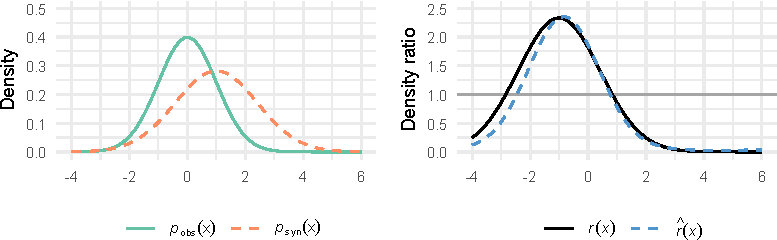
\includegraphics[width=1\linewidth,height=\textheight,keepaspectratio]{paper_files/figure-pdf/fig-dr-plot-1.pdf}

}

\caption{\label{fig-dr-plot}Example of the true and estimated density
ratio of two normal distributions with different means and variances
(i.e., \(\psyn(\bx) = N(0,1)\) and \(\pobs(\bx) = N(1,2)\)). The
function \(r(\bx) = \pobs(\bx)/\psyn(\bx)\) denotes the true density
ratio, the function \(\hat{r}(\bx)\) denotes an estimate of the density
ratio based on \(\nsyn = \nobs = 200\) samples from each distribution
obtained with unconstrained Least-Squares Importance Fitting (uLSIF).
Note that the density ratio is itself not a proper density.}

\end{figure}%

\linespread{2}

\subsubsection{Estimating the density
ratio}\label{estimating-the-density-ratio}

Over the past years, several methods for direct density ratio estimation
have been developed. A large class of these methods attempt to directly
minimize the error between the true density ratio \(r(\bx)\) and a
density ratio model \(\hat{r}(\bx)\). Following this approach, we define
a loss function \(\mathcal{L}(r(\bx), \hat{r}(\bx))\) that measures the
discrepancy between the true and estimated density ratio. To give an
example, consider the following loss based on the squared error
\begin{equation}\phantomsection\label{eq-squared-error}{
\begin{aligned}
\mathcal{L}^*_S(r(\bx), \hat{r}(\bx)) &= 
\frac{1}{2} \int (\hat{r}(\bx) - r(\bx))^2 \psyn(\bx) \text{d}\bx \\
&= \frac{1}{2} \int \hat{r}(\bx)^2 \psyn(\bx) \text{d}\bx - 
\int \hat{r}(\bx) r(\bx) \psyn(\bx) \text{d}\bx + 
\frac{1}{2} \int r(\bx)^2 \psyn(\bx) \text{d}\bx.
\end{aligned}
}\end{equation} The second term can be rewritten, because the
denominator in \(r(\bx)\) cancels with \(\psyn(\bx)\), while the third
term is a constant with respect to the parameters in the density ratio
model and can thus be ignored. Hence, we are left with the following
loss function to minimize
\begin{equation}\phantomsection\label{eq-squared-error-loss}{
\mathcal{L}_S (r(\bx), \hat{r}(\bx)) = \frac{1}{2} \int \hat{r}(\bx)^2 \psyn(\bx) \text{d}\bx - \int \hat{r}(\bx) \pobs(\bx) \text{d}\bx,
}\end{equation} which is termed least squares importance fitting (LSIF)
by Kanamori, Hido, and Sugiyama
(\citeproc{ref-kanamori_ulsif_2009}{2009}).

This approach can be straightforwardly generalized to a wide class of
loss functions that fall under the family of Bregman divergences (see
\citeproc{ref-sugiyama_bregman_2012}{Sugiyama, Suzuki, and Kanamori
2012b}; \citeproc{ref-mohamed2017learning}{Mohamed and Lakshminarayanan
2017}). Then, a general class of losses is encompassed by the expression
\begin{equation}\phantomsection\label{eq-bregman-loss}{
\mathcal{L}^*_f (r(\bx), \hat{r}(\bx)) =
\int \Big(
f(r(\bx)) - f(\hat{r}(\bx)) - f'(\hat{r}(\bx))(r(\bx) - \hat{r}(\bx))
\Big) \psyn(\bx) \text{d}\bx,
}\end{equation} where \(f\) is a differentiable and strictly convex
function with derivative \(f'\). Then, ignoring the terms independent of
\(\hat{r}(\bx)\) and noting that \(r(\bx)\psyn(\bx) = \pobs(\bx)\), we
obtain the following objective
\begin{equation}\phantomsection\label{eq-bregman-objective}{
\mathcal{L}_f (r(\bx), \hat{r}(\bx)) = \int 
\Big( 
f'(\hat{r}(\bx)) \hat{r}(\bx) - f(\hat{r}(\bx))
\Big)  \psyn(\bx) \text{d}\bx
- \int f'(\hat{r}(\bx)) \pobs(\bx)
\text{d}\bx.
}\end{equation} Minimizing this loss over \(\hat{r}(\bx)\) for different
functions \(f\) yields different estimators for the density ratio, that
focus on different regions of the density ratio.\footnote{It is easy to
  see that using \(f(x) = \frac{1}{2}(x-1)^2\) turns the Bregman
  divergence (Equation~\ref{eq-bregman-loss}) into the squared error
  (Equation~\ref{eq-squared-error}).} Specifically, some estimators
place more emphasis on accurately modelling the regions in which the
true density ratio is large, but less emphasis on accurately estimating
the density ratio in regions where it takes small values, and vice versa
(see \citeproc{ref-sugiyama_bregman_2012}{Sugiyama, Suzuki, and Kanamori
2012b}; \citeproc{ref-menon2016dreloss}{Menon and Ong 2016}).
Importantly, Sugiyama, Suzuki, and Kanamori
(\citeproc{ref-sugiyama_bregman_2012}{2012b}) show that the Bregman
divergence minimization approach to density ratio estimation is
equivalent to estimating an \(f\)-divergence
(\citeproc{ref-ali_silvey_divergence_1966}{Ali and Silvey 1966}) of the
observed data distribution from the synthetic data distribution. Hence,
when estimating the density ratio, one implicitly estimates the
divergence between the observed and synthetic data distributions.

After defining a loss function, we need a model for the density ratio
function \(\hat{r}(\bx)\). There are many possibilities to specify this
model, but a common choice is to use a linear model for the density
ratio (e.g., \citeproc{ref-huang_kmm_2006}{Huang et al. 2006};
\citeproc{ref-kanamori_ulsif_2009}{Kanamori, Hido, and Sugiyama 2009};
\citeproc{ref-izbicki_dre_2014}{Izbicki, Lee, and Schafer 2014};
\citeproc{ref-gruber2024overcoming}{Gruber et al. 2024}). That is, we
define the density ratio model as
\begin{equation}\phantomsection\label{eq-dr-model}{
\hat{r}(\bx) = \boldsymbol{\varphi}(\bx) \boldsymbol{\theta},
}\end{equation} where \(\boldsymbol{\varphi}(\bx)\) is a basis function
vector (optionally including an intercept term), that transforms the
data from a \(p\)-dimensional to a \(b\)-dimensional space, and
\(\boldsymbol{\theta}\) is a \(b\)-dimensional parameter vector.
Although the model is linear in its parameters, the density ratio itself
is typically a non-linear function of the data due to the basis
functions. The parameter vector \(\boldsymbol{\theta}\) is estimated to
minimize the discrepancy with the true density ratio using the loss
function \(\mathcal{L}(r(\bx), \hat{r}(\bx))\) in
Equation~\ref{eq-bregman-objective}. Potentially, the loss function can
be extended with a regularization term (e.g., a \(L_1\) or \(L_2\) norm
on the parameters of the model), to decrease the flexibility of the
density ratio.

Also for the basis functions, several specifications are possible,
ranging from an identity function
(\citeproc{ref-qin_inferences_1998}{Qin 1998}) to normalizing flows
(\citeproc{ref-choi_featurized_2021}{Choi, Liao, and Ermon 2021}) or
neural networks (\citeproc{ref-tiao2018dre}{Tiao 2018};
\citeproc{ref-uehara2016generative}{Uehara et al. 2016}). A commonly
used basis function in the density ratio literature is the Gaussian
kernel function (e.g., \citeproc{ref-huang_kmm_2006}{Huang et al. 2006};
\citeproc{ref-sugiyama_kliep_2007}{Sugiyama et al. 2007};
\citeproc{ref-kanamori_ulsif_2009}{Kanamori, Hido, and Sugiyama 2009};
\citeproc{ref-liu_change_2013}{Liu et al. 2013};
\citeproc{ref-gruber2024overcoming}{Gruber et al. 2024}). The Gaussian
kernel function is defined as \[
\boldsymbol{\varphi}(\bx) = \mathcal{K}(\bx, \boldsymbol{c}_j) = 
\exp\left(
- \frac{\lVert\bx - \boldsymbol{c}_j \rVert^2}{2 \sigma^2}
\right),
\] where \(\boldsymbol{c}_j\) (\(j \in 1, \dots, b\)) denotes the
centers of the Gaussian kernel functions, and \(\sigma\) controls the
kernel width (i.e., it defines over which distance similarity between
the observations and the centers are considered relevant; for more
information on kernel functions, see, e.g.,
\citeproc{ref-murphy_pmlintro_2022}{Murphy 2022}). The appropriate width
of the kernel and the optimal value of the regularization parameter can
be determined using cross-validation. The centers are typically sampled
from the data (in our case, both the observed and synthetic data).

After defining the model and the loss function, the density ratio can be
estimated. The \texttt{densityratio} package in R
(\citeproc{ref-densityratio}{Volker 2023}) provides an implementation of
commonly used loss functions with a Gaussian kernel basis function. The
package comes with an easy-to-use interface, automatic cross-validation
of hyperparameters and builds on \texttt{C++} for fast computation (see
Appendix \ref{sec-app-A} for a brief demonstration). Alternatively,
parameter estimation can be carried out using standard optimization
techniques (see Appendix \ref{sec-app-A} for a brief demonstration of
both approaches). The density ratio estimation framework thus equips
researchers with a measure of utility which is accurate, fast to compute
and does not require user specification of the model.

\subsubsection{Evaluating data utility with the density
ratio}\label{evaluating-data-utility-with-the-density-ratio}

Having estimated the density ratio, we can evaluate both global and
local utility of the synthetic data. Like other global utility measures,
the density ratio can be used to construct a single discrepancy measure
that quantifies the degree of misfit of the synthetic data. The density
ratio can be used to directly calculate some \(f\)-divergence between
the observed and synthetic data distributions, which serves as a measure
of utility for the synthetic data. Although this divergence statistic is
difficult to interpret in an absolute sense, it can be used as a
relative measure of the quality of the synthetic data. That is, for
different synthetic data sets, we can calculate the divergence to the
observed data, and compare these values to determine which synthetic
data set is most similar to the observed data. More formally, the
\(f\)-divergence can be used in a permutation test to determine whether
the synthetic data is generated from the same distribution as the
observed data. The corresponding \(p\)-value can be calculated by
comparing the observed divergence measure to the null distribution of
divergence measures obtained using random permutations of the observed
and synthetic data (see, for example,
\citeproc{ref-sugiyama_lstst_2011}{Sugiyama, Suzuki, et al. 2011};
\citeproc{ref-Wornowizki2016}{Wornowizki and Fried 2016};
\citeproc{ref-kanamori_divergence_2012}{Kanamori, Suzuki, and Sugiyama
2012a}).

An appealing characteristic of the density ratio framework is that it
also readily allows for evaluating local utility. As said, the estimated
density ratio shows in which regions the synthetic data diverges from
the observed data. By inspecting which observations have a high, or
small, estimated density ratio, we can identify the regions in which the
synthetic data is most different from the observed data. Visual
inspection can aid this process, for example by plotting the estimated
density ratio against variables or pairs of variables in the data. On an
even finer scale, the density ratio can be used to identify individual
observations that are far from what can be expected on the basis of the
observed data. This information could identify flaws in the synthetic
data model, or could be used directly to remove such observations from
the synthetic data. An additional advantage of the density ratio lies in
the fact that for every synthetic observation, the predicted density
ratio value can be regarded as an importance weight. Releasing the
predicted density ratio values for each synthetic observation allows
data users to reweigh analyses on the synthetic data. We illustrate
these features in Section~\ref{sec-app}.

A final advantage of the density ratio estimation framework lies in its
flexibility. The combination of a non-parametric kernel-based model with
automatic cross-validation for hyperparameter selection (e.g., kernel
and regularization parameters) allows for flexible estimation of the
density ratio. This flexibility reduces the burden on the user in terms
of model specification when evaluating the utility of the synthetic
data. All functionality described above, including visualization,
divergence estimation (and testing), extracting importance weights and
automatic cross-validation for hyperparameter selection, is readily
available in the \texttt{densityratio} \texttt{R}-package
(\citeproc{ref-densityratio}{Volker 2023}). The package provides fast
and efficient algorithms for density ratio estimation, and uses default
implementations that work across a wide range of data distributions,
which will be shown in the upcoming simulations.

\section{Numerical illustrations: Simulation
studies}\label{numerical-illustrations-simulation-studies}

To evaluate the performance of density ratio estimation and compare it
to existing methods, we conduct a series of simulation studies (all code
is available on GitHub\footnote{\url{https://github.com/thomvolker/dr-utility}}).
First, we illustrate the approach in a univariate simulation, after
which we evaluate the performance of the approach in a multivariate
setting, varying the distributions, number of variables and sample
sizes. To perform density ratio estimation, we use unconstrained
Least-Squares Importance Fitting (uLSIF;
\citeproc{ref-kanamori_ulsif_2009}{Kanamori, Hido, and Sugiyama 2009})
as implemented in the \texttt{densityratio} package in \texttt{R}
(\citeproc{ref-densityratio}{Volker 2023}), because it fast and has been
shown to perform well in a variety of settings (e.g.,
\citeproc{ref-kanamori_ulsif_2009}{Kanamori, Hido, and Sugiyama 2009};
\citeproc{ref-li_application_2010}{Li et al. 2010};
\citeproc{ref-Kanamori2012}{Kanamori, Suzuki, and Sugiyama 2012b}). We
compare the performance of uLSIF to the performance of state-of-the-art
software implementations of the \(pMSE\) (\citeproc{ref-synthpop}{Nowok,
Raab, and Dibben 2016}) and Kullback-Leibler divergence estimation
through \(k\)-nearest neighbor density estimation
(\citeproc{ref-kldest}{Hartung 2024}). Note that Kullback-Leibler
divergence estimation through \(k\)-nearest neighbor density estimation
implicitly performs direct density ratio estimation, and the procedure
can be regarded as a special case of density ratio estimation (see
Appendix \ref{sec-app-B}).

\subsection{Univariate illustrations}\label{sec-univ-sims}

We first illustrate the behavior of density ratio estimation in a
univariate setting, which simplifies visualization of the estimated
density ratios. Specifically, we consider four settings in which we
generate the real data from a distribution, and generate synthetic data
from an approximating Gaussian distribution with the same mean and
variance as the true data generating mechanism. The real data is
generated from (1) a Laplace distribution, (2) a log-normal
distribution, (3) a location-scale \(t\)-distribution and (4) a normal
distribution (see Figure~\ref{fig-densities-sim1}). Subsequently, we
approximate the true data generating mechanism using a Gaussian model
with the same mean and variance as the original data. This setting is
similar to situations commonly encountered in the synthetic data field,
in the sense that the true data generating mechanism is unknown and
needs to be approximated using a simpler approximating model. The exact
specifications of the data generating mechanisms are as follows:

\begin{enumerate}
\def\labelenumi{\arabic{enumi}.}
\tightlist
\item
  Laplace distribution with location parameter \(\mu = 1\) and scale
  \(b = 1\).
\item
  Log-normal distribution with log-mean
  \(\mu_{\text{log}} = \log \{1/\sqrt{3} \}\) and log-variance
  \(\sigma^2_\text{log} = \log 3\).
\item
  Location-scale \(t\)-distribution with location parameter \(\mu = 1\),
  scale \(\tau^2 = 1\) and degrees of freedom \(\nu = 4\).
\item
  Normal distribution with mean \(\mu = 1\) and variance
  \(\sigma^2 = 2\).
\end{enumerate}

These data generating mechanisms are chosen such that they all have the
same population mean \(\mu = 1\) and variance \(\sigma^2 = 2\). The
approximating Gaussian distribution has mean \(\mu = 1\) and variance
\(\sigma^2 = 2\). Hence, the synthetic data has the same population mean
and variance, but differs in higher-order moments, except in the fourth
scenario, where it is equal to true data generating mechanism. In all
scenarios, we generate \(1000\) data sets with \(\nobs = 250\)
observations from the true data generating mechanism, and
\(\nsyn = 250\) synthetic observations from the approximating Gaussian
model. The density ratio model is estimated using uLSIF with the default
Gaussian kernel and \(L_2\)-penalty on the parameter vector
\(\boldsymbol{\theta}\). Both the kernel bandwidth and the
regularization parameter are selected using cross-validation, using the
default settings in the \texttt{densityratio} package.

\linespread{1}

\begin{figure}[t]

\centering{

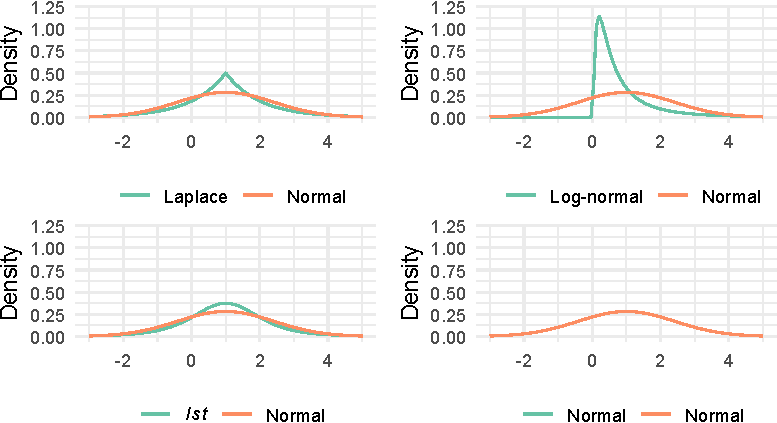
\includegraphics[width=1\linewidth,height=\textheight,keepaspectratio]{paper_files/figure-pdf/fig-densities-sim1-1.pdf}

}

\caption{\label{fig-densities-sim1}True and synthetic data densities for
the four simulations with Laplace, Log-normal, location-scale \(t\)- and
Normal densities. All data-generating mechanisms have the same mean
\(\mu = 1\) and variance \(\sigma^2 = 2\). Note that the true and
synthetic data density in the bottom right panel are completely
overlapping.}

\end{figure}%

\linespread{2}

\linespread{1}

\begin{figure}[t]

\centering{

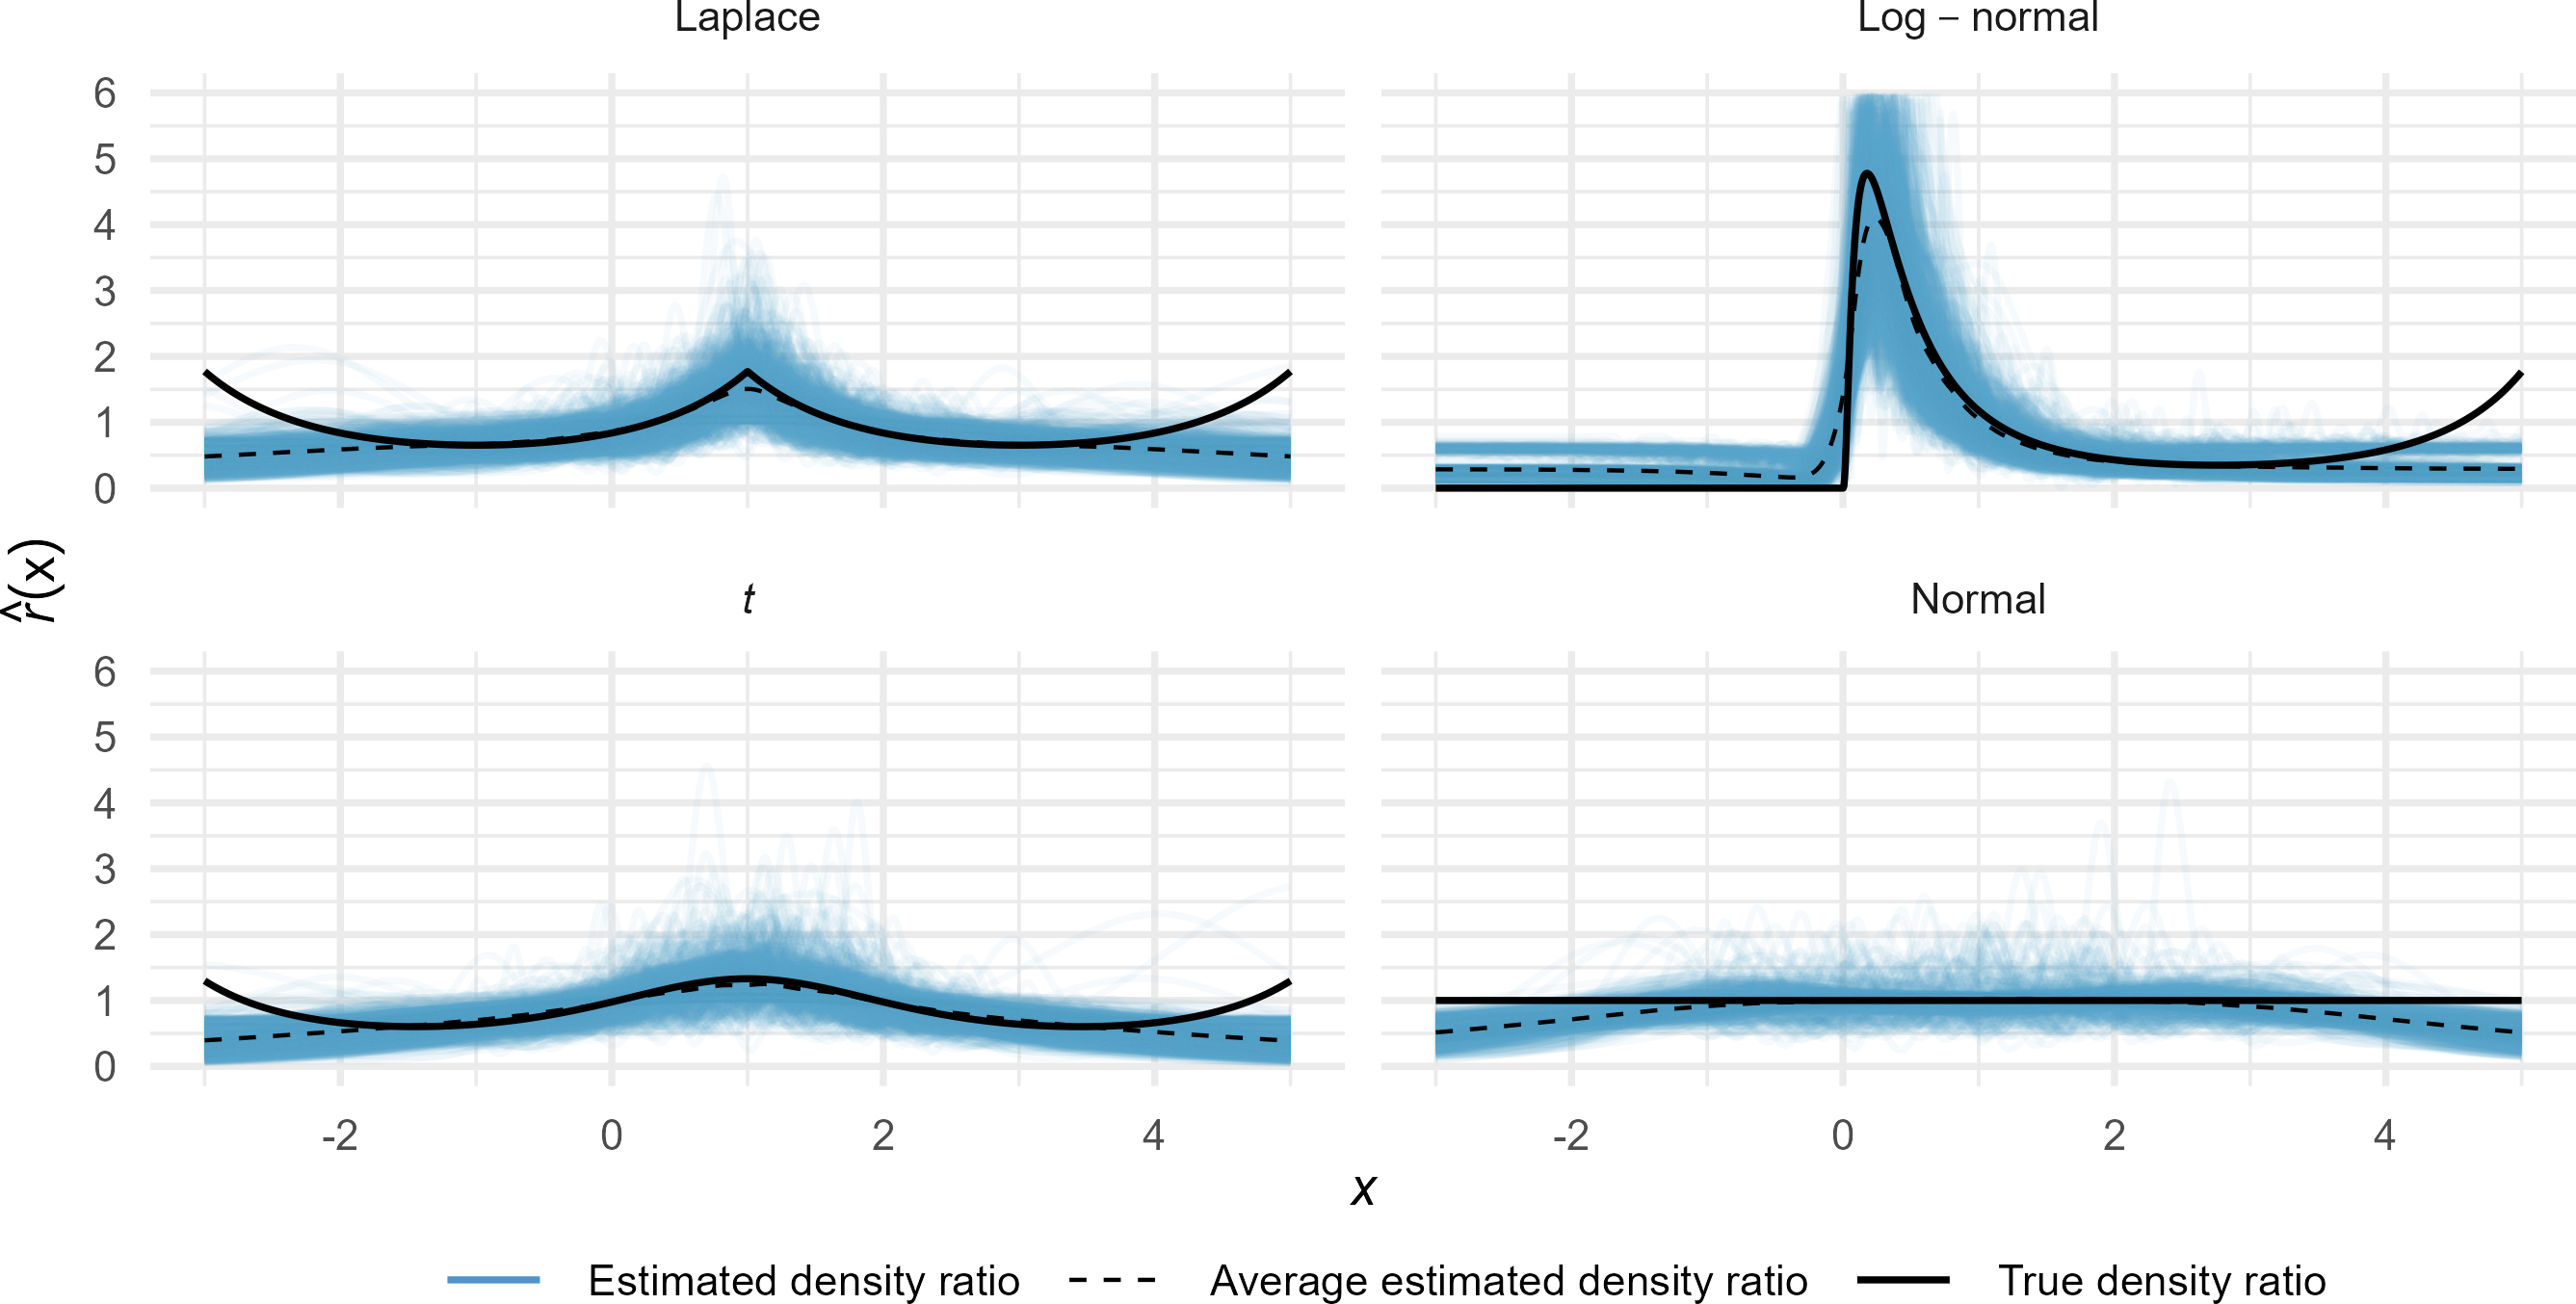
\includegraphics[width=1\linewidth,height=\textheight,keepaspectratio]{paper_files/figure-pdf/fig-sim1-results-1.png}

}

\caption{\label{fig-sim1-results}Estimated density ratios by
unconstrained least-squares importance fitting in four univariate
examples: A Laplace distribution, a log-normal distribution, a
location-scale \(t\)-distribution and a normal distribution, all
approximated by a normal distribution with the same mean and variance as
the sample from the true distribution. Note that the mass of the
synthetic data distribution in the tails (smaller than \(-2\) or greater
than \(4\)) is smaller than \(0.034\).}

\end{figure}%

\linespread{2}

Figure~\ref{fig-sim1-results} shows that the estimated density ratios
(the blue lines) follow the general trend of the true density ratio (the
solid black line) for each data-generating mechanism. Especially in the
center of each panel, approximately between \(-2\) and \(4\), the
average density ratio (the dashed black line) closely matches the true
density ratio. Moreover, all estimated density ratios model the peak in
the center of each panel, where the true data generating distribution
has more mass than the synthetic data distribution (except the bottom
right panel, where the true and synthetic data distributions are the
same). When moving from the middle to the sides, where the synthetic
data distribution has more mass than the true data generating
distributions, the estimated density ratios still follow the true
density ratios, in the sense that they are typically smaller than \(1\).
In the tails of the distribution, where the synthetic data distribution
has almost no mass (\(P(x \leq -2) = P(x \geq 4) \approx 0.017\)),
estimating the density ratio becomes difficult, leading to estimated
density ratios that diverge from the true density ratios In these
regions, the kernel function yields low values for most observations,
which, combined with the \(L_2\)-penalty on the density ratio
parameters, yields a downward bias for the estimated density ratio.

When assessing the panels individually, the following observations can
be made. In the top-left panel, showing the estimated density ratio of
the Laplace-distributed samples over the synthetic Gaussian-distributed
samples, the peak in the center is well approximated. Yet, the
discontinuity in the peak of the Laplace distribution cannot be captured
by a Gaussian kernel, which by definition models the density ratio as a
smooth function. The same can be said about the log-normal distribution,
where the cut-off at \(0\) is not captured exactly. Moreover, this panel
clearly shows the shrinkage due to the regularization parameter. When
there are no samples in one of the two distributions, the regularization
has relatively more influence and shrinks the density ratio parameters
towards zero. Accordingly, the estimated density ratio is shrunk towards
the estimated intercept parameter. The same behavior can be seen in the
bottom-left panel, showing the estimated density ratios of
location-scale \(t\)-distribution over the Gaussian samples. In the
centre of the distributions, the density ratio is well approximated, but
the density ratio is consistently underestimated in the tails of the
distribution. Lastly, it can be seen that, although the estimated
density ratios follow the general trends of the true density ratios,
there is also some variability around the true values, yielding rather
wiggly lines in some simulations.

Finally, we briefly compare the performance of uLSIF to \(k\)-nearest
neighbor density ratio estimation, which is implicitly used in
Kullback-Leibler divergence estimation through \(k\)-nearest neighbor
density estimation (see Appendix \ref{sec-app-B} for details). We set
the number of neighbors to \(k = 15 \approx \sqrt n\) (as suggested by
\citeproc{ref-loftsgaarden_nonparametric_1965}{Loftsgaarden and
Quesenberry 1965}). Figure~\ref{fig-AppB} shows that the estimated
density ratios by uLSIF are less variable than the estimated density
ratios by \(k\)-nearest neighbor density ratio estimation. Moreover, the
estimated density ratios by \(k\)-nearest neighbor density ratio
estimation have similar bias in the tails of the distribution, where
data is scarce. We conclude that uLSIF is able to provide more accurate
estimates of the density ratio if there are enough samples in the
regions of interest.

\subsection{Multivariate simulations}\label{multivariate-simulations}

To further investigate the performance of density ratio estimation, we
conducted a simulation study in a multivariate setting to compare
against existing global utility measures. The goal of these simulations
is to evaluate whether density ratio estimation is able to capture
improvements in the synthetic data model, and is able to reflect these
improvements in the utility statistics. In what follows, we describe the
data-generating mechanism, the synthetic data models, the utility
measures used to evaluate the quality of the synthetic data models and
the results of the simulations.

\subsubsection{True data-generating
mechanism}\label{true-data-generating-mechanism}

We generate the real data according to three data-generating mechanisms,
consisting of \(D \in \{5, 25, 50\}\) variables. When \(D = 5\), the
first four variables are multivariate normally distributed. These
normally distributed variables have mean \(\mu_d = 0\), variance
\(\sigma^2_{d,d} = 1\) and covariance \(\sigma^2_{d,d'} = 0.5\), for
\(d = 1, \dots, D-1\). The fifth variable is non-linearly related to the
first variable, such that
\(X_5 \sim \mathcal{N}(X_1^2, \hat{\text{Var}}(X_1^2))\). When
\(D = 25\) or \(D = 50\), the first \(20\) and \(45\) variables are
distributed normally, again with zero mean, unit variance and covariance
\(\sigma^2_{d,d'} = 0.5\) for \(d = 1, \dots, D-5\). The last five
variables have a non-linear relationship with the first five variables,
defined as
\(X_{D-5+j} \sim \mathcal{N}(X_j^{j+1}, \hat{\text{Var}}(X_j^j))\), for
\(j = 1, \dots, 5\). Hence, the first variable with a non-linear
relationship is obtained by raising the first variable to the power
\(2\), the second is obtained by raising the second variable to the
power \(3\), and so on, with an additional variance term that scales
with the variability due to raising terms to a higher power. For each
number of variables, we generate \(1000\) data sets, with three
different numbers of observations (\(n \in \{100, 1000, 2000\}\)).

\subsubsection{Synthetic data
generation}\label{synthetic-data-generation}

We generate synthetic data via three mechanisms, each incrementally
closer to the true data generating mechanism. The first synthetic data
model is a multivariate normal distribution with mean and variance
estimated from the real data, but neither covariances nor non-linear
relationships are taken into account. The second synthetic data model is
a multivariate normal distribution with means, variances and covariances
estimated from the real data, but without the non-linear relationships.
The final, and correctly specified, synthetic data model estimates the
means, variances, covariances and non-linear parameters from the data.
Each synthetic data set has the same number of observations as the
observed data.

\subsubsection{Utility measures}\label{utility-measures}

The goal of the simulation study is to evaluate whether the global
utility measures are able to detect the improvements in the synthesis
models. To this end, we use three different utility measures, and two
different specifications of each measure. First, we use uLSIF with
automatic hyperparameter selection through cross-validation (the default
in the \texttt{densityratio}-package). We summarize the estimated
utility of the synthetic data into a single number using the Pearson
divergence (\(PE\); \citeproc{ref-sugiyama_lstst_2011}{Sugiyama, Suzuki,
et al. 2011}). Additionally, we use the Kullback-Leibler divergence
based on \(k\)-nearest neighbor density ratio estimation as implemented
in the \texttt{R}-package \texttt{kldest} (\citeproc{ref-kldest}{Hartung
2024}), varying the number of neighbors between \(k = 1\) (the default
in the software) and \(k = \sqrt{n}\) (as advocated by
\citeproc{ref-loftsgaarden_nonparametric_1965}{Loftsgaarden and
Quesenberry 1965}). Finally, we use the \(pMSE\)-ratio, based on a CART
model using the default settings in \texttt{synthpop}
(\citeproc{ref-synthpop}{Nowok, Raab, and Dibben 2016}) and a logistic
regression model without interactions, as not all combinations of number
of variables and samples allow to include interactions in the model.

\subsubsection{Results}\label{results}

\linespread{1}

\begin{table}

\caption{\label{tbl-sim2-results}Proportion of simulations in which the
true synthetic data model order is captured by the utility measure. The
column \(PE\) refers to the Pearson divergence estimated using uLSIF,
\(KL_1\) and \(KL_{\sqrt{n}}\) refer to the Kullback-Leibler divergence
estimated using \(k\)-nearest neighbor density ratio estimation with
respectively \(k = 1\) and \(k = \sqrt{n}\), and \(pMSE_{\text{CART}}\)
and \(pMSE_{\text{logit}}\) refer to the \(pMSE\)-ratio estimated using
a CART model and a logistic regression model, respectively.
\vspace{0.4cm}}

\centering{

\centering
\begin{tabular}{ll>{\centering\arraybackslash}p{15mm}>{\centering\arraybackslash}p{15mm}>{\centering\arraybackslash}p{15mm}>{\centering\arraybackslash}p{15mm}>{\centering\arraybackslash}p{15mm}>{}p{15mm}}
\toprule
$n$ & $D$ & $PE$ & $KL_1$ & $KL_{\sqrt{n}}$ & $pMSE_{\text{CART}}$ & $pMSE_{\text{logit}}$\\
\midrule
100 & 5 & 0.583 & 0.844 & 0.904 & 0.362 & 0.188\\
100 & 25 & 0.450 & 0.838 & 0.933 & 0.368 & 0.250\\
100 & 50 & 0.363 & 0.673 & 0.786 & 0.352 & 0.352\\
\addlinespace
1000 & 5 & 1.000 & 1.000 & 1.000 & 0.885 & 0.173\\
1000 & 25 & 1.000 & 1.000 & 1.000 & 0.898 & 0.242\\
1000 & 50 & 0.997 & 1.000 & 1.000 & 0.839 & 0.316\\
\addlinespace
2000 & 5 & 1.000 & 1.000 & 1.000 & 0.882 & 0.173\\
2000 & 25 & 1.000 & 1.000 & 1.000 & 0.816 & 0.247\\
2000 & 50 & 1.000 & 1.000 & 1.000 & 0.780 & 0.324\\
\bottomrule
\end{tabular}

}

\end{table}%

\linespread{2}

Table~\ref{tbl-sim2-results} shows the proportion of simulations in
which the utility measures correctly order the synthetic data sets in
terms of quality of the synthesis model. That is, the first synthesis
model, using only the means and variances of each variable, should have
the lowest utility (highest divergence or \(pMSE\)-ratio), followed by
the second synthesis model, using the correct means, variances and
covariances but not the non-linear relationships, and the third,
correctly specified synthesis model should obtain the highest utility
score. Table~\ref{tbl-sim2-results} shows that the \(KL\)-divergence
based on \(k = \sqrt{n}\) neighbors correctly ranks the synthetic data
sets most often, followed by the \(KL\)-divergence based on \(k = 1\)
neighbors and the uLSIF model. Unless the sample size is small, these
approaches correctly rank the synthetic data sets in almost all
instances. Both the \(KL\)-divergence and the density ratio based
Pearson divergence clearly outperform the common \(pMSE\). Additionally,
Table~\ref{tbl-sim2-results} shows that the performance of all utility
measures improves with the sample size, and decreases when the
dimensionality of the data increases. The only exception to the latter
trend is the logistic regression based \(pMSE\)-ratio model, which
consistently improves with the dimensionality of the data).

To zoom in on the behavior of the three methods, we visualize the
results of uLSIF, the \(KL\)-divergence based on \(k = \sqrt{n}\)
neighbors, and the \(pMSE\)-ratio based on a CART model for \(n = 1000\)
and \(D = 50\) in Figure~\ref{fig-sim2-results}. For \(PE\) and
\(KL_{\sqrt{n}}\), the improvements in the synthesis model are
consistently picked up by the utility measures, whereas for
\(pMSE_\text{cart}\), the estimated changes in utility are much more
variable across the simulations. Additionally, the figures show that the
improvement in utility due to modelling the covariances rather than only
the means and variances is much larger than the improvement due to also
modelling the non-linear relationships. That is, the increase in utility
is much more pronounced when moving from the first to the second
synthetic data set than moving from the second to the third synthetic
data set.

\linespread{1}

\begin{figure}[t]

\centering{

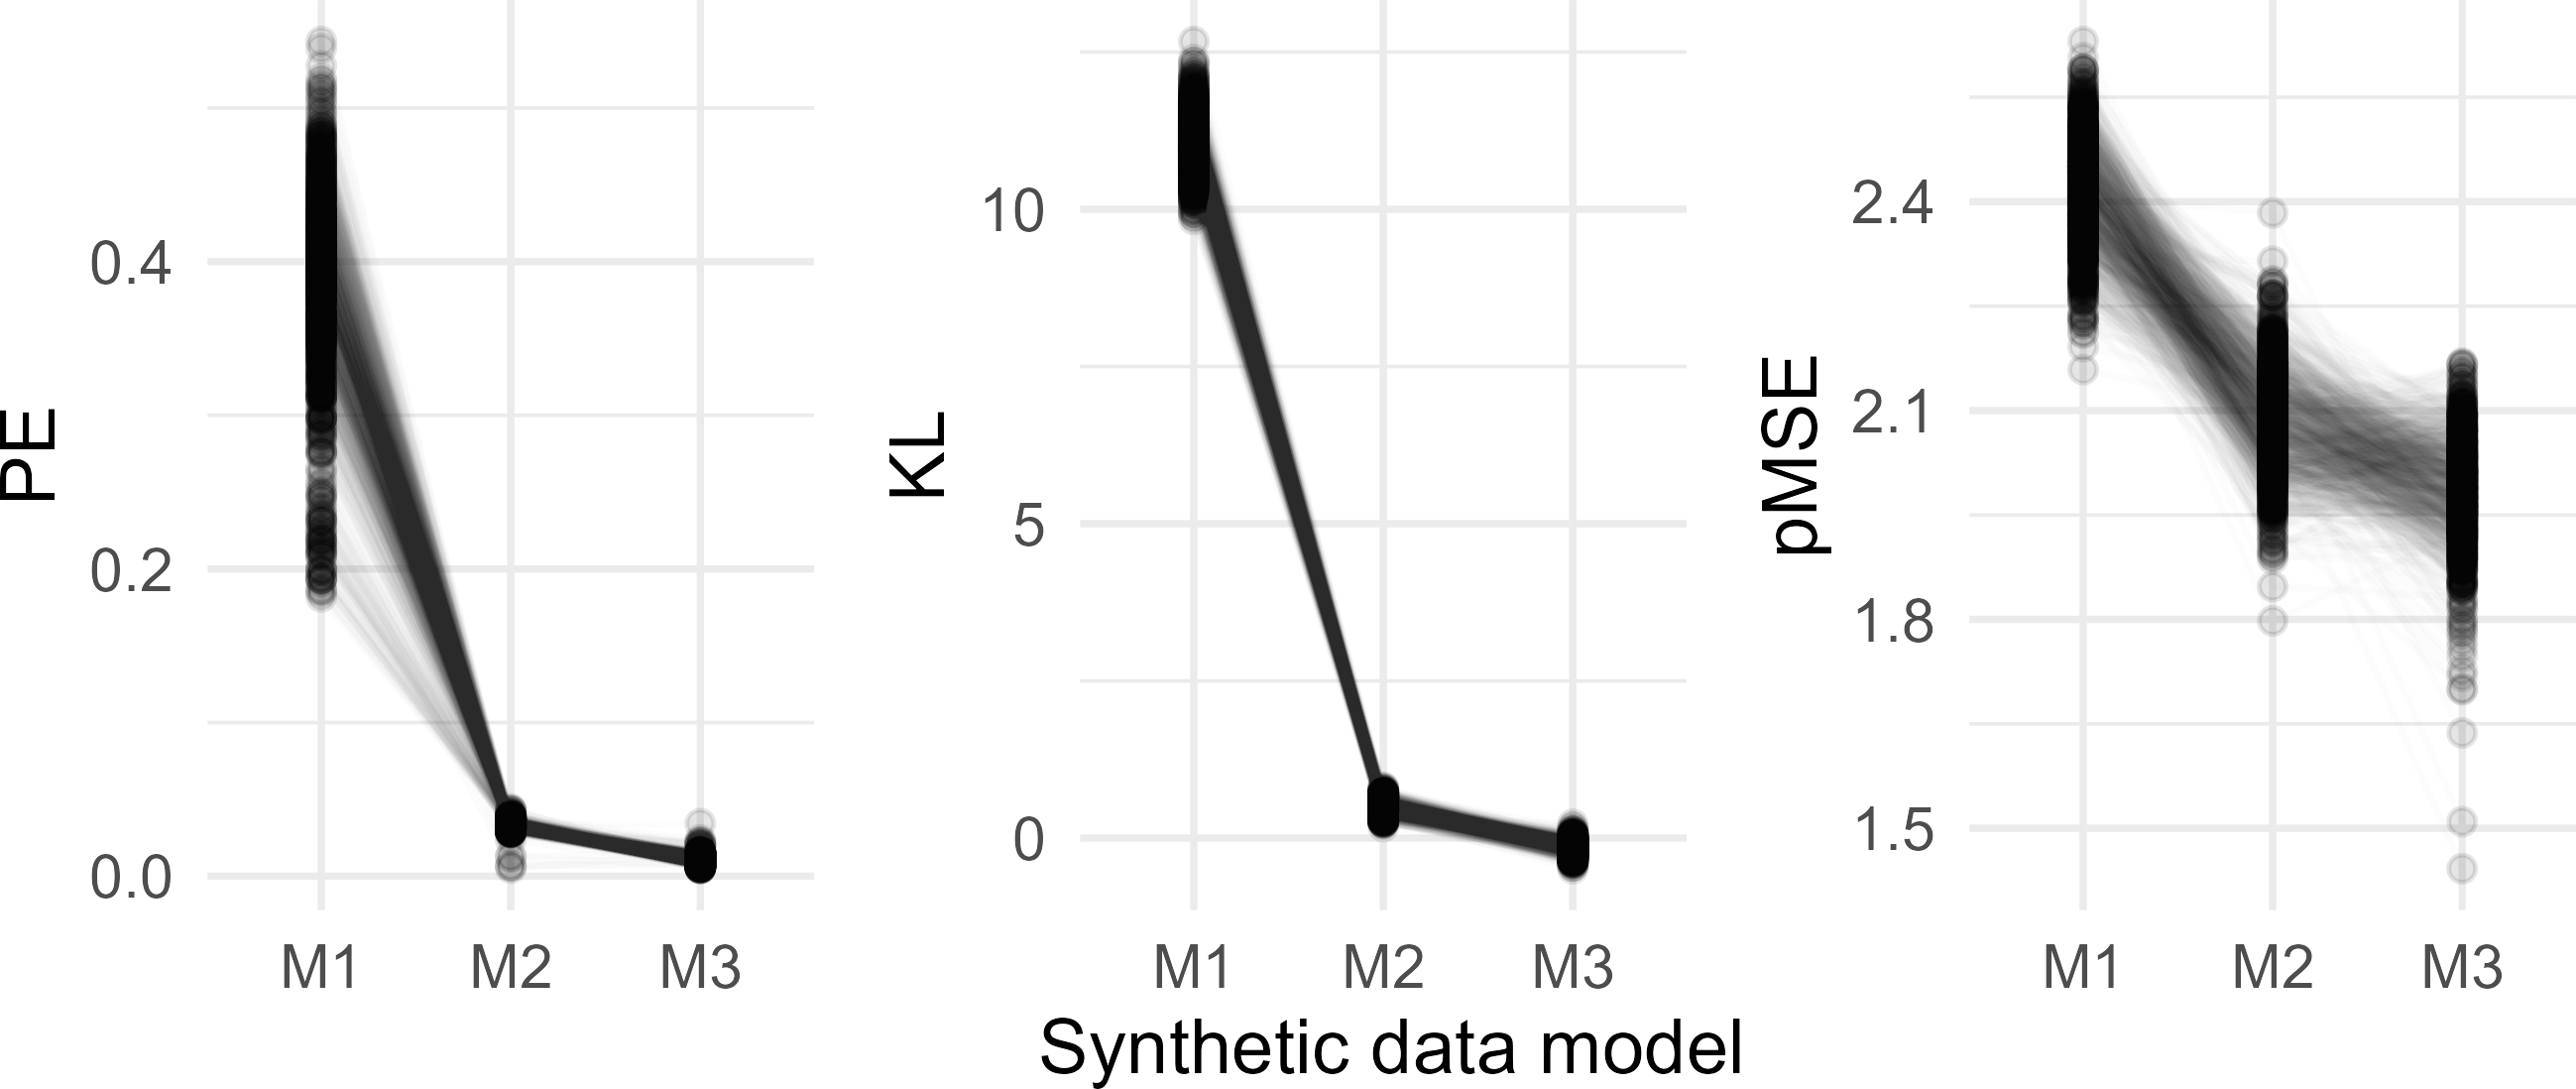
\includegraphics[width=1\linewidth,height=\textheight,keepaspectratio]{paper_files/figure-pdf/fig-sim2-results-1.png}

}

\caption{\label{fig-sim2-results}The estimated utility measures (\(PE\),
\(KL_{\sqrt{n}}\) and \(pMSE_{\text{cart}}\)) for \(n = 1000\)
observations and \(D = 25\) variables in \(1000\) simulations for the
three increasingly accurate synthetic data models. All metrics show how
the estimated utility improves with the refinements of the synthesis
models, but \(PE\) and \(KL_{\sqrt{n}}\) show less variability and catch
the synthesis model improvements more consistently.}

\end{figure}%

\linespread{2}

These results have a remarkable implication for the evaluation of
synthetic data generation methods. When the aim is to rank candidate
synthetic data sets using a global utility statistic, using a rather
flexible model seems advisable. In Section~\ref{sec-univ-sims} and
Appendix \ref{sec-app-B}, we showed that the \(k\)-nearest neighbor
density ratio estimate is substantially more variable than the
uLSIF-based estimate, but when the aim is to quantify the utility of the
synthetic data, this variability does not seem to be problematic.
Rather, these simulations seem to suggest that a more flexible model is
better able to detect discrepancies between the observed and synthetic
data. Obtaining a stable and accurate estimate of the density ratio (or,
by analogy, of the propensity scores in the \(pMSE\)) does not seem to
be required when one is solely interested in globally ranking different
synthetic data sets. However, local information on the misfit of the
synthetic data is valuable in itself, which we illustrate in the next
section.

\section{Application: Synthetic data generation for the U.S. Current
Population Survey}\label{sec-app}

\linespread{1}

\linespread{2}

To further illustrate the use of density ratio estimation for synthetic
data utility using the March 2000 U.S. Current Population Survey (CPS).
The data contains the continuous variables age, household income,
household property taxes and social security payments, and the
categorical variables sex, race, marital status and education level
measured on \(n_\text{obs} = 5000\) individuals. We compare two
different synthesis strategies that increasingly tailor toward the data
at hand (using the \texttt{R}-package \texttt{synthpop};
\citeproc{ref-synthpop}{Nowok, Raab, and Dibben 2016}). Note that all
continuous variables except age are substantially skewed. Moreover, the
variables household property taxes and social security payments have a
point-mass at zero (see the first column in
Figure~\ref{fig-application-distributions}). To account for the
skewness, we transform the continuous variables to cubic root scale
(\(f(x) = |x|^{1/3}\cdot\text{sign}(x)\)). Accordingly, the first
modelling strategies applies a linear regression model on the
transformed continuous variables. The categorical variables are modelled
using (multinomial) logistic regression models. The second modelling
strategy extends the first strategy by applying a semi-continuous model
to the transformed variables household property taxes and social
security payments. Here, the point mass is modelled first using a
logistic regression model, after which the non-zero values are
synthesized using a linear regression model. All other variables are
modelled according to the first strategy. We generate \(m = 5\)
synthetic data sets for both strategies, each with
\(n_\text{syn} = 5000\) observations, and evaluate their utility using
unconstrained least-squares importance fitting. We emphasize that
throughout the illustration, we use the same default settings as in the
previous sections.

\subsection{Evaluating global utility using density ratio
estimation}\label{evaluating-global-utility-using-density-ratio-estimation}

\linespread{1}

\begin{figure}[t]

\centering{

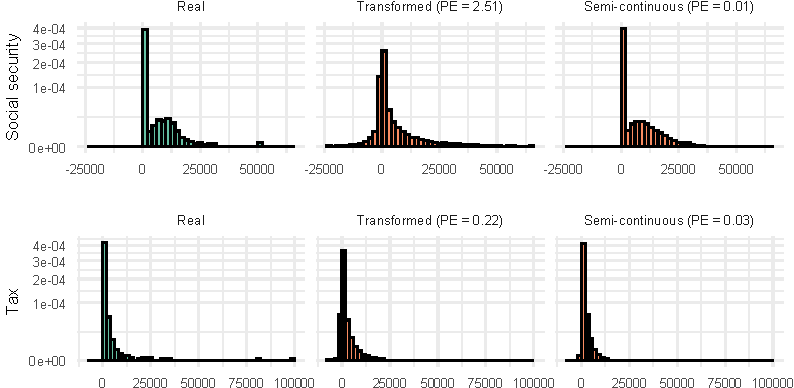
\includegraphics[width=1\linewidth,height=\textheight,keepaspectratio]{paper_files/figure-pdf/fig-application-distributions-1.pdf}

}

\caption{\label{fig-application-distributions}Real and synthetic data
distributions for the variables household property taxes and social
security benefits (social security) for the transformed and
semi-continuous synthesis strategy. The panel titles display the
estimated Pearson divergence for each variable between the observed and
synthetic data, estimated using a density ratio model for each variable
separately. Note that the y-axis is displayed on a square-root scale to
enhance visibility.}

\end{figure}%

\linespread{2}

Figure~\ref{fig-application-distributions} displays the distributions of
the variables social security payments (Social security) and household
property taxes (Tax) for the real data and the synthetic data according
to the transformed and semi-continuous modelling strategies. The figure
shows that the semi-continuous modelling strategy fits the observed data
better than the transformed modelling strategy, as it better captures
the point mass and does not yield an excessive number of negative
values. Note that there are only minor differences for the other
variables, as there are no differences in synthesis methods. When
evaluating the global utility of the two synthetic data sets, the
improvement in synthesis models is reflected in the Pearson divergence.
That is, the transformed modelling strategy has a higher average
estimated Pearson divergence (\(\bar{PE}_\text{transformed} = 0.085\),
\(\text{range} = [0.080, 0.091]\)) than the semi-continuous modelling
strategy (\(\bar{PE}_\text{semi-continuous} = 0.047\),
\(\text{range} = [0.044, 0.050]\)). Although the difference may seem
small in an absolute sense, it is substantial in a relative sense.
Additionally, the variability in estimated Pearson divergences for each
synthesis strategy is much smaller than the difference between the two
strategies. Finally, we remark that when estimating the density ratio on
the level of the individual variables, the semi-continuous modelling
strategy obtains substantially lower Pearson divergences than the
transformed modelling strategy see the panel titles in
Figure~\ref{fig-application-distributions}. Hence, we conclude that the
Pearson divergence serves as an adequate measure of synthetic data
utility.

\subsection{Density ratios as local utility
estimates}\label{density-ratios-as-local-utility-estimates}

\linespread{1}

\begin{figure}[t]

\centering{

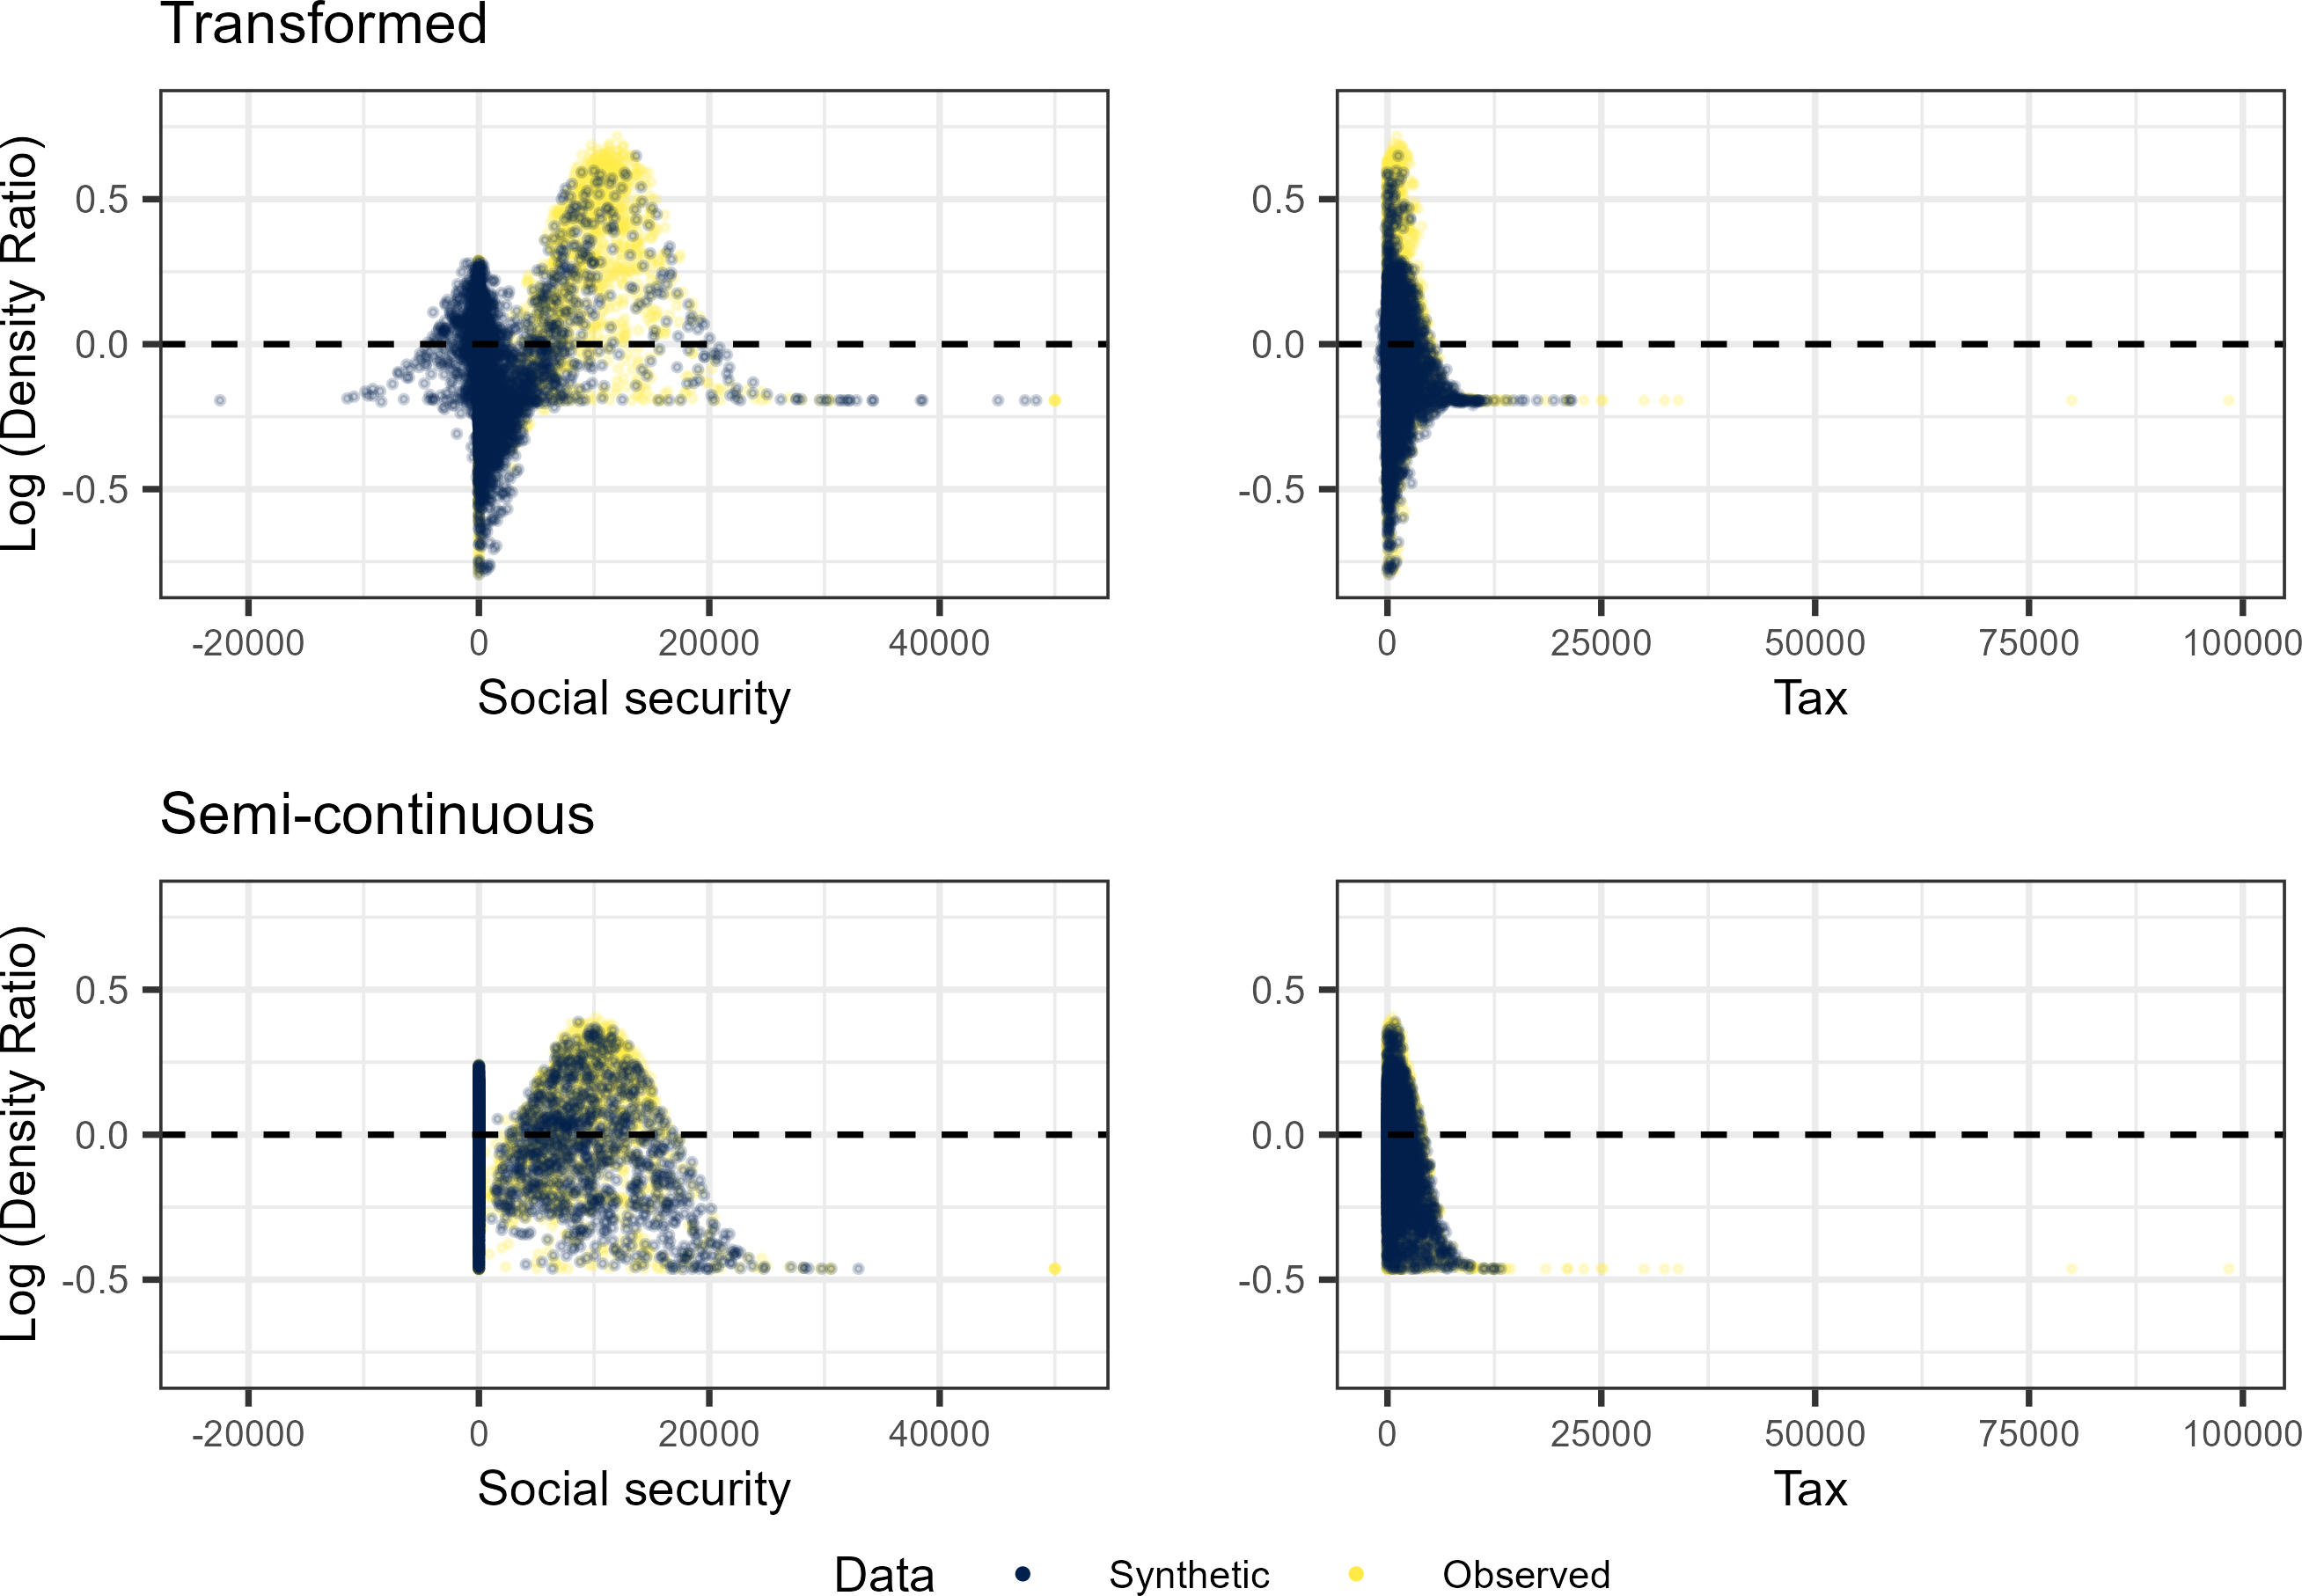
\includegraphics[width=1\linewidth,height=\textheight,keepaspectratio]{paper_files/figure-pdf/fig-app-utility-results-1.png}

}

\caption{\label{fig-app-utility-results}Estimated density ratios (on
log-scale) for the first synthetic data set under the two synthesis
strategies plotted against the variables social security payments
(Social security) and household property taxes (Tax) for the observed
and synthetic data. Note that the density ratios are estimated using a
single model for the entire data set.}

\end{figure}%

\linespread{2}

Besides quantifying the global utility of synthetic data, the density
ratio also provides local information about the utility of synthetic
data. First, the estimated density ratio can provide an intuition about
which variables are not modelled adequately. That is, by plotting the
estimated density ratio against each variable or pairs of variables, one
can identify variables for which there is a clear pattern in the density
ratio values. Figure~\ref{fig-app-utility-results} shows the estimated
density ratio values (on a log-scale) for the variables social security
payments and household property taxes for the first synthetic data set
under both synthesis strategies. First, the figure shows that the spread
in density ratio values is substantially larger for the transformed
modelling strategy than for the semi-continuous modelling strategy.
Second, the estimated density ratios indicate that the transformed
modelling strategy misses the point mass at zero for social security,
but generated too many values slightly larger than zero. Moreover,
figure shows that the transformed modelling strategy yielded too little
mass at the values around \(10000\), as indicated by the spike in
density ratio values around \(10000\). Plotting the density ratio
against household property taxes is less insightful, as the difference
in marginal distributions is relatively small. For the semi-continuous
modelling strategy, there is some spread in density ratio values, but
there is no clear pattern, and the synthetic and observed data points
are mostly overlapping. Hence, marginally, the density ratio values do
not reveal a substantial misfit of the semi-continuous strategy.

Additionally, we note that in the tails of the distribution, the
estimated density ratios are regularized, such that the high values for
tax in the observed data do not yield extremely high density ratio
values. From a utility perspective, this might be undesirable, as misfit
in the tails of the distribution might go by unnoticed. However, from a
privacy perspective, this regularization is beneficial, as it prevents
the density ratio from becoming very large around the location of
outlying observed data points, potentially revealing the location of
these points. The regularization thus ensures that the density ratio is
not overly sensitive to individual observations.

Finally, we illustrate another use of the density ratio as a local
utility measure, namely, using the density ratio as importance weights
in downstream analysis tasks. In this case, we consider the synthetic
data as a sample that suffers from selection bias, and we use the
estimated density ratio as importance weights to correct for this bias
when making inferences. Using importance weighting after density ratio
estimation, it is possible to obtain consistent estimates of the
population parameters (\citeproc{ref-kanamori_ulsif_2009}{Kanamori,
Hido, and Sugiyama 2009}; \citeproc{ref-Kanamori2012}{Kanamori, Suzuki,
and Sugiyama 2012b}), even when the synthesis method is not consistent.
Consider the case that we deem our semi-continuous synthetic data model
sufficient from both a privacy and utility perspective. Perhaps using
more complex synthesis models would yield higher utility, but at the
cost of a higher disclosure risk. To further improve the utility of the
semi-continuous synthetic data, we can release the estimated density
ratio values, such that a third-party can use these values as importance
weights in their analysis. Releasing these weights obviously adds to the
disclosure risk as more information about the observed data is provided.
However, the density ratio values might be less disclosive then
synthetic data generated with a more complex synthesis model. Although
this is no formal guarantee, the regularization in the density ratio
model limits the influence each observation has on the density ratio
values. We return to this issue in the discussion.

\linespread{1}

\begin{table}

\caption{\label{tbl-application-regression}Linear regression
coefficients for the observed data, synthetic data and reweighted
synthetic data using the density ratio as importance weights. Boldface
text indicates which coefficient has smaller absolute bias relative to
the observed data.}

\centering{

\begin{tabular}{lrll}
\toprule
Variable & Observed & Synthetic & Reweighted\\
\midrule
Intercept & 10.297 & \textbf{10.192} & 10.182\\
Age & -0.003 & -0.005 & \textbf{-0.004}\\
Education: High school & 0.283 & 0.415 & \textbf{ 0.397}\\
Education: Associate or Bachelor's degree & 0.593 & 0.782 & \textbf{ 0.744}\\
Education: Master's degree or higher & 1.016 & 1.135 & \textbf{ 1.092}\\
Marital: Separated & -0.500 & \textbf{-0.434} & -0.433\\
Marital: Widowed & -0.467 & \textbf{-0.471} & -0.448\\
Marital: Single & -0.491 & -0.592 & \textbf{-0.561}\\
Marital: Widowed or divorced & -0.549 & \textbf{-0.518} & -0.505\\
Race: Non-white & -0.090 & \textbf{-0.109} & -0.110\\
Sex: Female & -0.117 & -0.134 & \textbf{-0.126}\\
log(Tax + 1) & 0.067 & 0.071 & \textbf{ 0.067}\\
log(Social security + 1) & -0.026 & -0.009 & \textbf{-0.016}\\
\bottomrule
\end{tabular}

}

\end{table}%

\linespread{2}

To demonstrate the idea, we fit a linear regression model predicting the
logarithm of household income using all predictors in the data set
(i.e., age, household property taxes, social security payments, sex,
race, marital status and education level) on the observed data and the
semi-continuous synthetic data. Subsequently, we estimate the model on
the semi-continuous synthetic data using the estimated density ratio
values as importance weights. Table~\ref{tbl-application-regression}
shows the coefficients of these regression models averaged over the
\(m=5\) synthetic datasets, where boldface text denotes the coefficient
with smallest absolute bias compared to the estimate obtained from the
observed data. The table shows that although the synthetic regression
coefficients are quite close to the observed data coefficients, the
reweighed coefficients further improve the accuracy. Especially for the
continuous predictors, age, household property taxes and social security
payments, using the density ratio weights improves the estimates.
Averaging the absolute normalized bias over all coefficients and all
synthetic data sets yields an improvement from approximately
\(\text{avg}(|\beta_\text{obs}-\beta_\text{syn}|/SE_\text{obs}) = 1.98\)
to
\(\text{avg}(|\beta_\text{obs}-\beta_\text{syn-adj}|/SE_\text{obs}) = 1.54\)
after reweighing. Hence, besides providing a measure of global utility,
the estimated density ratio can be used to further improve the utility
of the synthetic data.

\section{Discussion and conclusion}\label{discussion-and-conclusion}

High quality utility measures are essential when creating synthetic data
for use in downstream tasks. These measures provide an insight into the
quality of the synthetic data, and can be used to guide the synthesis
process, fostering higher quality synthetic data. In this paper, we
provided a framework for evaluating synthetic data utility through
density ratio estimation. Our simulations and illustration show that the
density estimation framework can be used in a wide variety of settings,
and yields more accurate results than established procedures for
evaluating synthetic data utility under a variety of synthetic data
models and sample sizes, all using the same default hyperparameter
specifications. Moreover, we showed that the estimated density ratio,
besides providing a global utility measure, serves as a measure of local
utility, and can even be used directly to further improve specific
utility of the synthetic data. We have made these methods openly
available through the \texttt{densityratio} package in \texttt{R}
(\citeproc{ref-densityratio}{Volker 2023}).

Throughout the paper, we have contrasted the density ratio framework
with existing utility measures as the \(pMSE\) and the Kullback-Leibler
divergence. Both measures can be considered special cases of the density
ratio framework. The Kullback-Leibler divergence explicitly contains the
density ratio in its definition, and Appendix \ref{sec-app-B} describes
how the \(k\)-nearest neighbor approach to \(KL\)-divergence estimation
gives rise to a direct estimate of the density ratio. The \(pMSE\) can
also be seen as a special case of the density ratio framework, by noting
that the predicted probabilities are easily transformed into density
ratios (see \citeproc{ref-sugiyama_suzuki_kanamori_2012}{Sugiyama,
Suzuki, and Kanamori 2012a}). In fact, Menon and Ong
(\citeproc{ref-menon2016dreloss}{2016}) show that density ratio
estimation is equivalent to class probability estimation (as performed
in the \(pMSE\)), in the sense that minimizing a class probability
estimation loss is equivalent to minimizing a Bregman divergence to the
true density ratio function. These connections raise the question which
model class, and which loss function, is most appropriate when the goal
is to evaluate the utility of synthetic data.

While we leave a formal evaluation of this question to future work, we
can provide some intuitions. First, utility measures ought to be robust,
in the sense that they should not be too sensitive to extreme values in
the observed data, as this may pose a privacy risk. That is, extreme
cases typically bear higher disclosure risk as they do not blend into
the crowd (\citeproc{ref-gehrke_crowd_2012}{Gehrke et al. 2012}). If the
utility measure is too sensitive to these extreme cases, small
discrepancies that serve to protect privacy may seem to reflect low
quality synthetic data. Sugiyama, Suzuki, and Kanamori
(\citeproc{ref-sugiyama_bregman_2012}{2012b}) showed that uLSIF is
relatively robust to outliers compared to density ratio estimation using
the \(KL\)-loss, but the robustness can further be improved by using
different loss functions (such as Basu's power divergence;
\citeproc{ref-basu_power_1998}{Basu et al. 1998}). Second, utility
measures should work well in a wide-variety of settings, so users do not
need to fine-tune utility measures and focus on the problem at hand. To
this end, non-parametric methods may be preferred over parametric
methods, as they do not hinge upon an appropriate model specification.
Although correctly specified parametric models are more efficient in a
statistical sense, they are less reliable when the model is misspecified
(\citeproc{ref-sugiyama_suzuki_kanamori_2012}{Sugiyama, Suzuki, and
Kanamori 2012a}). Throughout the paper, we have shown that uLSIF serves
as a suitable compromise between flexibility and robustness, although
the KL-divergence using \(k\)-nearest neighbor density ratio estimation
may be more sensitive to discrepancies between the observed and
synthetic data.

By viewing synthetic data utility through the lens of density ratio
estimation, several appealing properties are obtained. First, the
density ratio perspective encompasses global and local utility in a
single framework. The estimated density ratio gives rise to global
utility measures, but also allows for the identification of variables
that have not been modelled adequately. Additionally, the estimated
density ratio can be used directly to improve the utility of the
synthetic data, by reweighing the synthetic data to better match the
observed data. These findings are supported by other research showing
that synthetic data utility can be improved by importance weighting
(\citeproc{ref-ghalebikesabi_dpiw_2022}{Ghalebikesabi et al. 2022}). The
proposed framework provide a flexible class of models that are easily
implemented through the \texttt{densityratio} package
(\citeproc{ref-densityratio}{Volker 2023}), that tailor to a wide
variety of settings. Moreover, several extensions are available to deal
with high-dimensional data, enabling the evaluation of the quality of
synthetic data with many variables, such as spectral density ratio
estimation (\citeproc{ref-izbicki_dre_2014}{Izbicki, Lee, and Schafer
2014}) and least-squares heterodistributional subspace search
(\citeproc{ref-sugiyama_lhss_2011}{Sugiyama, Yamada, et al. 2011}), both
implemented in the \texttt{densityratio} package. Finally, the framework
can be used directly to create synthetic data, as the density ratio can
serve the role of discriminator in generative models
(\citeproc{ref-uehara2016generative}{Uehara et al. 2016}).

Despite the appealing characteristics of density ratio estimation,
several open questions remain. Kernel methods, as typically employed in
density ratio estimation, can be sensitive to the choice of kernel, and
the use of a Gaussian kernel, while a reasonable and versatile default,
may not be appropriate in every situation. Categorical variables, for
instance, are not naturally incorporated in the current set-up. To deal
with this issue, we created dummy variables for the categories of the
categorical variables in our illustration, which provided reasonable
results. However, other solutions (i.e., different kernels or distance
measures) may lead to improvements. Additionally, our results showed
that the current approach to regularization is not ideal, as the density
ratio estimates are shrunk towards an estimated intercept. However, when
the intercept deviates from one, the numerator or denominator density
are up or downweighted. Rather, one would like to shrink the density
ratio estimates towards one, as this is more in line with the
interpretation that there is no information to estimate the density
ratio. Finally, releasing information from the density ratio may pose an
additional privacy risk, as it leaks additional information about the
original data. Presumably, solely releasing a global utility measure,
such as the Pearson divergence, will yield only additional risk.
Releasing the density ratio values themselves may, however, pose
unacceptable privacy risks, especially when the density ratio model is
sensitive to extreme cases. Privatizing density ratio estimation
presents an interesting avenue for future research.

Despite these open questions, we have shown that already in its current
form, density ratio estimation provides a flexible and informative
framework for evaluating synthetic data utility. Due to its in-built
model selection, it requires little specification on behalf of the user
and works well in a wide variety of settings. The framework can be
readily incorporated into synthetic data workflows using the
\texttt{densityratio} package.

\section*{Acknowledgements}\label{acknowledgements}
\addcontentsline{toc}{section}{Acknowledgements}

We are grateful to Joerg Drechsler for sharing the U.S. Current
Population Survey data, and to Stef van Buuren, Gerko Vink, Hanne
Oberman and Carlos Gonzalez Poses for many valuable discussions.

\section*{References}\label{references}
\addcontentsline{toc}{section}{References}

\phantomsection\label{refs}
\begin{CSLReferences}{1}{0}
\bibitem[\citeproctext]{ref-SIPP_Beta_2006}
Abowd, John M., Martha Stinson, and Gary Benedetto. 2006. {``Final
Report to the Social Security Administration on the {SIPP/SSA/IRS}
Public Use File Project.''} Longitudinal Employer-Household Dynamics
Program, U.S. Bureau of the Census, Washington, DC.
\url{https://ecommons.cornell.edu/bitstream/handle/1813/43929/SSAfinal.pdf?sequence=3&isAllowed=y}.

\bibitem[\citeproctext]{ref-ali_silvey_divergence_1966}
Ali, S. M., and S. D. Silvey. 1966. {``A General Class of Coefficients
of Divergence of One Distribution from Another.''} \emph{Journal of the
Royal Statistical Society. Series B (Methodological)} 28 (1): 131--42.
\url{https://doi.org/10.1111/j.2517-6161.1966.tb00626.x}.

\bibitem[\citeproctext]{ref-atenas_open_2015}
Atenas, Javiera, Leo Havemann, and Ernesto Priego. 2015. {``Open Data as
Open Educational Resources: Towards Transversal Skills and Global
Citizenship.''} \emph{Open Praxis} 7 (4): 377--89.
\url{https://www.learntechlib.org/p/161986}.

\bibitem[\citeproctext]{ref-basu_power_1998}
Basu, Ayanendranath, Ian R. Harris, Nils L. Hjort, and M. C. Jones.
1998. {``{Robust and efficient estimation by minimising a density power
divergence}.''} \emph{Biometrika} 85 (3): 549--59.
\url{https://doi.org/10.1093/biomet/85.3.549}.

\bibitem[\citeproctext]{ref-Bowen_differentially_2021}
Bowen, Claire McKay, Fang Liu, and Bingyue Su. 2021. {``Differentially
Private Data Release via Statistical Election to Partition
Sequentially.''} \emph{METRON} 79 (1): 1--31.
\url{https://doi.org/10.1007/s40300-021-00201-0}.

\bibitem[\citeproctext]{ref-choi_featurized_2021}
Choi, Kristy, Madeline Liao, and Stefano Ermon. 2021. {``Featurized
Density Ratio Estimation.''} In \emph{Proceedings of the Thirty-Seventh
Conference on Uncertainty in Artificial Intelligence}, edited by Cassio
de Campos and Marloes H. Maathuis, 161:172--82. Proceedings of Machine
Learning Research. PMLR.
\url{https://proceedings.mlr.press/v161/choi21a.html}.

\bibitem[\citeproctext]{ref-crosas_automating_2015}
Crosas, Mercè, Gary King, James Honaker, and Latanya Sweeney. 2015.
{``Automating Open Science for Big Data.''} \emph{The ANNALS of the
American Academy of Political and Social Science} 659 (1): 260--73.
\url{https://doi.org/10.1177/0002716215570847}.

\bibitem[\citeproctext]{ref-drechsler2011synthetic}
Drechsler, Jörg. 2011. \emph{Synthetic Datasets for Statistical
Disclosure Control: Theory and Implementation}. New York: Springer
Science \& Business Media.
\url{https://doi.org/10.1007/978-1-4614-0326-5}.

\bibitem[\citeproctext]{ref-drechsler2012}
---------. 2012. {``New Data Dissemination Approaches in Old Europe
{\textendash} Synthetic Datasets for a German Establishment Survey.''}
\emph{Journal of Applied Statistics} 39 (2): 243--65.
\url{https://doi.org/10.1080/02664763.2011.584523}.

\bibitem[\citeproctext]{ref-drechsler_utility_2022}
---------. 2022. {``Challenges in Measuring Utility for Fully Synthetic
Data.''} In \emph{Privacy in Statistical Databases}, edited by Josep
Domingo-Ferrer and Maryline Laurent, 220--33. Cham: Springer
International Publishing.
\url{https://doi.org/10.1007/978-3-031-13945-1_16}.

\bibitem[\citeproctext]{ref-drechsler2023}
Drechsler, Jörg, and Anna-Carolina Haensch. 2023. {``30 Years of
Synthetic Data.''} \url{https://doi.org/10.48550/ARXIV.2304.02107}.

\bibitem[\citeproctext]{ref-Rcpp}
Eddelbuettel, Dirk. 2013. \emph{Seamless {R} and {C++} Integration with
{Rcpp}}. New York: Springer.
\url{https://doi.org/10.1007/978-1-4614-6868-4}.

\bibitem[\citeproctext]{ref-gdpr}
European Parliament, and Council of the European Union. 2016.
{``Regulation ({EU}) 2016/679 of the {European} {Parliament} and of the
{Council}. Of 27 {April} 2016 on the Protection of Natural Persons with
Regard to the Processing of Personal Data and on the Free Movement of
Such Data, and Repealing {Directive} 95/46/{EC} ({General} {Data}
{Protection} {Regulation}).''} OJ L 119, 4.5.2016, p. 1--88. May 4,
2016. \url{https://eur-lex.europa.eu/eli/reg/2016/679/oj}.

\bibitem[\citeproctext]{ref-fpf_2017}
Future of Privacy Forum. 2017. {``Understanding Corporate Data Sharing
Decisions: Practices, Challenges, and Opportunities for Sharing
Corporate Data with Researchers.''}

\bibitem[\citeproctext]{ref-gehrke_crowd_2012}
Gehrke, Johannes, Michael Hay, Edward Lui, and Rafael Pass. 2012.
{``Crowd-Blending Privacy.''} In \emph{Advances in Cryptology -- CRYPTO
2012}, edited by Reihaneh Safavi-Naini and Ran Canetti, 479--96. Berlin,
Heidelberg: Springer Berlin Heidelberg.
\url{https://doi.org/10.1007/978-3-642-32009-5_28}.

\bibitem[\citeproctext]{ref-ghalebikesabi_dpiw_2022}
Ghalebikesabi, Sahra, Harry Wilde, Jack Jewson, Arnaud Doucet, Sebastian
Vollmer, and Chris Holmes. 2022. {``Mitigating Statistical Bias Within
Differentially Private Synthetic Data.''} In \emph{Proceedings of the
Thirty-Eighth Conference on Uncertainty in Artificial Intelligence},
edited by James Cussens and Kun Zhang, 180:696--705. Proceedings of
Machine Learning Research. PMLR.
\url{https://proceedings.mlr.press/v180/ghalebikesabi22a.html}.

\bibitem[\citeproctext]{ref-gruber2024overcoming}
Gruber, Lukas, Markus Holzleitner, Johannes Lehner, Sepp Hochreiter, and
Werner Zellinger. 2024. {``Overcoming Saturation in Density Ratio
Estimation by Iterated Regularization.''}
\url{https://doi.org/10.48550/arXiv.2402.13891}.

\bibitem[\citeproctext]{ref-kldest}
Hartung, Niklas. 2024. \emph{Kldest: Sample-Based Estimation of
Kullback-Leibler Divergence}.
\url{https://CRAN.R-project.org/package=kldest}.

\bibitem[\citeproctext]{ref-hawala_synthetic_2008}
Hawala, Sam. 2008. \emph{Producing Partially Synthetic Data to Avoid
Disclosure}.
\url{http://www.asasrms.org/Proceedings/y2008/Files/301018.pdf}.

\bibitem[\citeproctext]{ref-shohei_dre_outlier_2008}
Hido, Shohei, Yuta Tsuboi, Hisashi Kashima, Masashi Sugiyama, and
Takafumi Kanamori. 2008. {``Inlier-Based Outlier Detection via Direct
Density Ratio Estimation.''} In \emph{2008 Eighth IEEE International
Conference on Data Mining}, edited by Fosca Giannotti, Dimitrios
Gunopulos, Franco Turini, Carlo Zaniolo, Naren Ramakrishnan, and Xindong
Wu, 223--32. \url{https://doi.org/10.1109/ICDM.2008.49}.

\bibitem[\citeproctext]{ref-hu_advancing_2024}
Hu, Jingchen, and Claire McKay Bowen. 2024. {``Advancing Microdata
Privacy Protection: A Review of Synthetic Data Methods.''} \emph{WIREs
Computational Statistics} 16 (1): e1636.
https://doi.org/\url{https://doi.org/10.1002/wics.1636}.

\bibitem[\citeproctext]{ref-huang_kmm_2006}
Huang, Jiayuan, Alexander J. Smola, Arthur Gretton, Karsten M.
Borgwardt, and Bernhard Schölkopf. 2006. {``Correcting Sample Selection
Bias by Unlabeled Data.''} In \emph{Advances in Neural Information
Processing Systems}, edited by B. Schölkopf, J. Platt, and T. Hoffman.
Vol. 19. MIT Press.
\url{https://proceedings.neurips.cc/paper_files/paper/2006/file/a2186aa7c086b46ad4e8bf81e2a3a19b-Paper.pdf}.

\bibitem[\citeproctext]{ref-hundepool_disclosure_2012}
Hundepool, Anco, Josep Domingo-Ferrer, Luisa Franconi, Sarah Giessing,
Eric Schulte Nordholt, Keith Spicer, and Peter-Paul De Wolf. 2012.
\emph{Statistical Disclosure Control}. John Wiley \& Sons.
\url{https://doi.org/10.1002/9781118348239}.

\bibitem[\citeproctext]{ref-izbicki_dre_2014}
Izbicki, Rafael, Ann Lee, and Chad Schafer. 2014. {``{High-Dimensional
Density Ratio Estimation with Extensions to Approximate Likelihood
Computation}.''} In \emph{Proceedings of the Seventeenth International
Conference on Artificial Intelligence and Statistics}, edited by Samuel
Kaski and Jukka Corander, 33:420--29. Proceedings of Machine Learning
Research. Reykjavik, Iceland: PMLR.
\url{https://proceedings.mlr.press/v33/izbicki14.html}.

\bibitem[\citeproctext]{ref-kanamori_ulsif_2009}
Kanamori, Takafumi, Shohei Hido, and Masashi Sugiyama. 2009. {``A
Least-Squares Approach to Direct Importance Estimation.''} \emph{Journal
of Machine Learning Research} 10 (48): 1391--1445.
\url{http://jmlr.org/papers/v10/kanamori09a.html}.

\bibitem[\citeproctext]{ref-kanamori_divergence_2012}
Kanamori, Takafumi, Taiji Suzuki, and Masashi Sugiyama. 2012a. {``\(f\)
-Divergence Estimation and Two-Sample Homogeneity Test Under
Semiparametric Density-Ratio Models.''} \emph{IEEE Transactions on
Information Theory} 58 (2): 708--20.
\url{https://doi.org/10.1109/TIT.2011.2163380}.

\bibitem[\citeproctext]{ref-Kanamori2012}
---------. 2012b. {``Statistical Analysis of Kernel-Based Least-Squares
Density-Ratio Estimation.''} \emph{Machine Learning} 86 (3): 335--67.
\url{https://doi.org/10.1007/s10994-011-5266-3}.

\bibitem[\citeproctext]{ref-karr_utility_2006}
Karr, Alan F., Christine N. Kohnen, Anna Oganian, Jerome P. Reiter, and
Ashish P. Sanil. 2006. {``A Framework for Evaluating the Utility of Data
Altered to Protect Confidentiality.''} \emph{The American Statistician}
60 (3): 224--32. \url{https://doi.org/10.1198/000313006X124640}.

\bibitem[\citeproctext]{ref-kim_classification_2021}
Kim, Ilmun, Aaditya Ramdas, Aarti Singh, and Larry Wasserman. 2021.
{``{Classification accuracy as a proxy for two-sample testing}.''}
\emph{The Annals of Statistics} 49 (1): 411--34.
\url{https://doi.org/10.1214/20-AOS1962}.

\bibitem[\citeproctext]{ref-lazer_css_2009}
Lazer, David, Alex Pentland, Lada Adamic, Sinan Aral, Albert-László
Barabási, Devon Brewer, Nicholas Christakis, et al. 2009.
{``Computational Social Science.''} \emph{Science} 323 (5915): 721--23.
\url{https://doi.org/10.1126/science.1167742}.

\bibitem[\citeproctext]{ref-li_application_2010}
Li, Yan, Hiroyuki Kambara, Yasuharu Koike, and Masashi Sugiyama. 2010.
{``Application of Covariate Shift Adaptation Techniques in
Brain--Computer Interfaces.''} \emph{IEEE Transactions on Biomedical
Engineering} 57 (6): 1318--24.
\url{https://doi.org/10.1109/TBME.2009.2039997}.

\bibitem[\citeproctext]{ref-little_statistical_1993}
Little, Roderick J. A. 1993. {``Statistical Analysis of Masked Data.''}
\emph{Journal of Official Statistics} 9 (2): 407--7.
\url{https://www.scb.se/contentassets/ca21efb41fee47d293bbee5bf7be7fb3/statistical-analysis-of-masked-data.pdf}.

\bibitem[\citeproctext]{ref-liu_change_2013}
Liu, Song, Makoto Yamada, Nigel Collier, and Masashi Sugiyama. 2013.
{``Change-Point Detection in Time-Series Data by Relative Density-Ratio
Estimation.''} \emph{Neural Networks} 43: 72--83.
\url{https://doi.org/10.1016/j.neunet.2013.01.012}.

\bibitem[\citeproctext]{ref-loftsgaarden_nonparametric_1965}
Loftsgaarden, D. O., and C. P. Quesenberry. 1965. {``{A Nonparametric
Estimate of a Multivariate Density Function}.''} \emph{The Annals of
Mathematical Statistics} 36 (3): 1049--51.
\url{https://doi.org/10.1214/aoms/1177700079}.

\bibitem[\citeproctext]{ref-menon2016dreloss}
Menon, Aditya, and Cheng Soon Ong. 2016. {``Linking Losses for Density
Ratio and Class-Probability Estimation.''} In \emph{Proceedings of the
33rd International Conference on Machine Learning}, edited by Maria
Florina Balcan and Kilian Q. Weinberger, 48:304--13. Proceedings of
Machine Learning Research. New York, New York, USA: PMLR.
\url{https://proceedings.mlr.press/v48/menon16.html}.

\bibitem[\citeproctext]{ref-mohamed2017learning}
Mohamed, Shakir, and Balaji Lakshminarayanan. 2017. {``Learning in
Implicit Generative Models.''}
\url{https://doi.org/10.48550/arXiv.1610.03483}.

\bibitem[\citeproctext]{ref-murphy_pmlintro_2022}
Murphy, Kevin P. 2022. \emph{Probabilistic Machine Learning: An
Introduction}. MIT Press. \href{https://probml.ai}{probml.ai}.

\bibitem[\citeproctext]{ref-newman_future_2012}
Newman, Greg, Andrea Wiggins, Alycia Crall, Eric Graham, Sarah Newman,
and Kevin Crowston. 2012. {``The Future of Citizen Science: Emerging
Technologies and Shifting Paradigms.''} \emph{Frontiers in Ecology and
the Environment} 10 (6): 298--304. \url{https://doi.org/10.1890/110294}.

\bibitem[\citeproctext]{ref-synthpop}
Nowok, Beata, Gillian M. Raab, and Chris Dibben. 2016.
{``{\emph{Synthpop}:} Bespoke Creation of Synthetic Data in
{\emph{R}}.''} \emph{Journal of Statistical Software} 74 (11).
\url{https://doi.org/10.18637/jss.v074.i11}.

\bibitem[\citeproctext]{ref-obels_analysis_2020}
Obels, Pepijn, Daniël Lakens, Nicholas A. Coles, Jaroslav Gottfried, and
Seth A. Green. 2020. {``Analysis of Open Data and Computational
Reproducibility in Registered Reports in Psychology.''} \emph{Advances
in Methods and Practices in Psychological Science} 3 (2): 229--37.
\url{https://doi.org/10.1177/2515245920918872}.

\bibitem[\citeproctext]{ref-obermeyer2019}
Obermeyer, Ziad, Brian Powers, Christine Vogeli, and Sendhil
Mullainathan. 2019. {``Dissecting Racial Bias in an Algorithm Used to
Manage the Health of Populations.''} \emph{Science} 366 (6464): 447--53.
\url{https://doi.org/10.1126/science.aax2342}.

\bibitem[\citeproctext]{ref-qin_inferences_1998}
Qin, Jing. 1998. {``{Inferences for case-control and semiparametric
two-sample density ratio models}.''} \emph{Biometrika} 85 (3): 619--30.
\url{https://doi.org/10.1093/biomet/85.3.619}.

\bibitem[\citeproctext]{ref-raab2017guidelines}
Raab, Gillian M., Beata Nowok, and Chris Dibben. 2017. {``Guidelines for
Producing Useful Synthetic Data.''}
\url{https://arxiv.org/abs/1712.04078}.

\bibitem[\citeproctext]{ref-raab2021assessing}
Raab, Gillian M, Beata Nowok, and Chris Dibben. 2021. {``Assessing,
Visualizing and Improving the Utility of Synthetic Data.''}
\url{https://doi.org/10.48550/arXiv.2109.12717}.

\bibitem[\citeproctext]{ref-ramachandran_open_2021}
Ramachandran, Rahul, Kaylin Bugbee, and Kevin Murphy. 2021. {``From Open
Data to Open Science.''} \emph{Earth and Space Science} 8 (5):
e2020EA001562. \url{https://doi.org/10.1029/2020EA001562}.

\bibitem[\citeproctext]{ref-reiter_releasing_2004}
Reiter, Jerome P. 2004. {``{Releasing Multiply Imputed, Synthetic Public
use Microdata: An Illustration and Empirical Study}.''} \emph{Journal of
the Royal Statistical Society Series A: Statistics in Society} 168 (1):
185--205. \url{https://doi.org/10.1111/j.1467-985X.2004.00343.x}.

\bibitem[\citeproctext]{ref-rubin_statistical_1993}
Rubin, Donald B. 1993. {``Statistical Disclosure Limitation.''}
\emph{Journal of Official Statistics} 9 (2): 461--68.
\url{https://www.scb.se/contentassets/ca21efb41fee47d293bbee5bf7be7fb3/discussion-statistical-disclosure-limitation2.pdf}.

\bibitem[\citeproctext]{ref-Scott1992}
Scott, David W. 1992. \emph{Multivariate Density Estimation: Theory,
Practice, and Visualization}. Wiley.
\url{https://doi.org/10.1002/9780470316849}.

\bibitem[\citeproctext]{ref-snoke_utility_2018}
Snoke, Joshua, Gillian M. Raab, Beata Nowok, Chris Dibben, and
Aleksandra Slavkovic. 2018. {``General and Specific Utility Measures for
Synthetic Data.''} \emph{Journal of the Royal Statistical Society.
Series A (Statistics in Society)} 181 (3): pp. 663--688.
\url{https://doi.org/10.1111/rssa.12358}.

\bibitem[\citeproctext]{ref-sugiyama_classification_2010}
Sugiyama, Masashi. 2010. {``Superfast-Trainable Multi-Class
Probabilistic Classifier by Least-Squares Posterior Fitting.''}
\emph{IEICE Transactions on Information and Systems} E93-D (10).
\url{https://doi.org/10.1587/transinf.E93.D.2690}.

\bibitem[\citeproctext]{ref-sugiyama_kliep_2007}
Sugiyama, Masashi, Shinichi Nakajima, Hisashi Kashima, Paul Buenau, and
Motoaki Kawanabe. 2007. {``Direct Importance Estimation with Model
Selection and Its Application to Covariate Shift Adaptation.''} In
\emph{Advances in Neural Information Processing Systems}, edited by J.
Platt, D. Koller, Y. Singer, and S. Roweis. Vol. 20. Curran Associates,
Inc.
\url{https://proceedings.neurips.cc/paper_files/paper/2007/file/be83ab3ecd0db773eb2dc1b0a17836a1-Paper.pdf}.

\bibitem[\citeproctext]{ref-sugiyama_lstst_2011}
Sugiyama, Masashi, Taiji Suzuki, Yuta Itoh, Takafumi Kanamori, and
Manabu Kimura. 2011. {``Least-Squares Two-Sample Test.''} \emph{Neural
Networks} 24 (7): 735--51.
\url{https://doi.org/10.1016/j.neunet.2011.04.003}.

\bibitem[\citeproctext]{ref-sugiyama_suzuki_kanamori_2012}
Sugiyama, Masashi, Taiji Suzuki, and Takafumi Kanamori. 2012a.
\emph{Density Ratio Estimation in Machine Learning}. Cambridge
University Press. \url{https://doi.org/10.1017/CBO9781139035613}.

\bibitem[\citeproctext]{ref-sugiyama_bregman_2012}
---------. 2012b. {``Density-Ratio Matching Under the Bregman
Divergence: A Unified Framework of Density-Ratio Estimation.''}
\emph{Annals of the Institute of Statistical Mathematics} 64 (5):
1009--44. \url{https://doi.org/10.1007/s10463-011-0343-8}.

\bibitem[\citeproctext]{ref-sugiyama_conditional_2010}
Sugiyama, Masashi, Ichiro Takeuchi, Taiji Suzuki, Takafumi Kanamori,
Hirotaka Hachiya, and Daisuke Okanohara. 2010. {``Conditional Density
Estimation via Least-Squares Density Ratio Estimation.''} In
\emph{Proceedings of the Thirteenth International Conference on
Artificial Intelligence and Statistics}, edited by Yee Whye Teh and Mike
Titterington, 9:781--88. Proceedings of Machine Learning Research. Chia
Laguna Resort, Sardinia, Italy: PMLR.
\url{https://proceedings.mlr.press/v9/sugiyama10a.html}.

\bibitem[\citeproctext]{ref-sugiyama_lhss_2011}
Sugiyama, Masashi, Makoto Yamada, Paul von Bünau, Taiji Suzuki, Takafumi
Kanamori, and Motoaki Kawanabe. 2011. {``Direct Density-Ratio Estimation
with Dimensionality Reduction via Least-Squares Hetero-Distributional
Subspace Search.''} \emph{Neural Networks} 24 (2): 183--98.
\url{https://doi.org/10.1016/j.neunet.2010.10.005}.

\bibitem[\citeproctext]{ref-tiao2018dre}
Tiao, Louis C. 2018. {``{D}ensity {R}atio {E}stimation for {KL}
{D}ivergence {M}inimization Between {I}mplicit {D}istributions.''}
\emph{Tiao.io}.
\url{https://tiao.io/post/density-ratio-estimation-for-kl-divergence-minimization-between-implicit-distributions/}.

\bibitem[\citeproctext]{ref-uehara2016generative}
Uehara, Masatoshi, Issei Sato, Masahiro Suzuki, Kotaro Nakayama, and
Yutaka Matsuo. 2016. {``Generative Adversarial Nets from a Density Ratio
Estimation Perspective.''}
\url{https://doi.org/10.48550/arXiv.1610.02920}.

\bibitem[\citeproctext]{ref-vandewiel2023}
van de Wiel, Mark A., Gwenaël G. R. Leday, Jeroen Hoogland, Martijn W.
Heymans, Erik W. van Zwet, and Ailko H. Zwinderman. 2023. {``Think
Before You Shrink: Alternatives to Default Shrinkage Methods Can Improve
Prediction Accuracy, Calibration and Coverage.''}
\url{https://doi.org/10.48550/ARXIV.2301.09890}.

\bibitem[\citeproctext]{ref-densityratio}
Volker, Thom Benjamin. 2023. {``Densityratio: Direct Estimation of the
Ratio of Densities of Two Groups of Observations.''}
\url{https://github.com/thomvolker/densityratio}.

\bibitem[\citeproctext]{ref-wang_divergence_2009}
Wang, Qing, Sanjeev R. Kulkarni, and Sergio Verdu. 2009. {``Divergence
Estimation for Multidimensional Densities via \(k\)-Nearest-Neighbor
Distances.''} \emph{IEEE Transactions on Information Theory} 55 (5):
2392--2405. \url{https://doi.org/10.1109/TIT.2009.2016060}.

\bibitem[\citeproctext]{ref-willenborg_elements_2001}
Willenborg, Leon, and Ton De Waal. 2001. \emph{Elements of Statistical
Disclosure Control}. Springer Science \& Business Media.
\url{https://doi.org/10.1007/978-1-4613-0121-9}.

\bibitem[\citeproctext]{ref-Woo_global_2009}
Woo, Mi-Ja, Jerome P. Reiter, Anna Oganian, and Alan F. Karr. 2009.
{``Global Measures of Data Utility for Microdata Masked for Disclosure
Limitation.''} \emph{Journal of Privacy and Confidentiality} 1 (1).
\url{https://doi.org/10.29012/jpc.v1i1.568}.

\bibitem[\citeproctext]{ref-Wornowizki2016}
Wornowizki, Max, and Roland Fried. 2016. {``Two-Sample Homogeneity Tests
Based on Divergence Measures.''} \emph{Computational Statistics} 31 (1):
291--313. \url{https://doi.org/10.1007/s00180-015-0633-3}.

\bibitem[\citeproctext]{ref-xu_ctgan_2019}
Xu, Lei, Maria Skoularidou, Alfredo Cuesta-Infante, and Kalyan
Veeramachaneni. 2019. \emph{Modeling Tabular Data Using Conditional
GAN}. Edited by H. Wallach, H. Larochelle, A. Beygelzimer, F.
dAlché-Buc, E. Fox, and R. Garnett. Vol. 32. Curran Associates, Inc.
\url{https://proceedings.neurips.cc/paper_files/paper/2019/file/254ed7d2de3b23ab10936522dd547b78-Paper.pdf}.

\bibitem[\citeproctext]{ref-zettler2021}
Zettler, Ingo, Christoph Schild, Lau Lilleholt, Lara Kroencke, Till
Utesch, Morten Moshagen, Robert Böhm, Mitja D. Back, and Katharina
Geukes. 2021. {``The Role of Personality in COVID-19-Related
Perceptions, Evaluations, and Behaviors: Findings Across Five Samples,
Nine Traits, and 17 Criteria.''} \emph{Social Psychological and
Personality Science} 13 (1): 299--310.
\url{https://doi.org/10.1177/19485506211001680}.

\end{CSLReferences}

\setcounter{section}{0}
\renewcommand{\thesection}{\Alph{section}}

\setcounter{table}{0}
\renewcommand{\thetable}{A\arabic{table}}

\setcounter{figure}{0}
\renewcommand{\thefigure}{A\arabic{figure}}

\section{\texorpdfstring{Density ratio estimation in
\texttt{R}}{Density ratio estimation in R}}\label{sec-app-A}

To perform density ratio estimation in \texttt{R}, we can use the
\texttt{densityratio} package, which includes model fitting functions
for multiple popular loss functions. Additionally, we can complement the
package with standard optimization routines in \texttt{R}. Here, we show
an example of both approaches.

We generate two small toy datasets, \texttt{x} and \texttt{y}, that
serve as numerator and denominator data, respectively. Moreover, we set
\texttt{x} as the centers in the Gaussian kernel, and we pre-define the
kernel bandwidth to be \(\sigma = 1\) and fix the regularization
parameter to \(\lambda = 0.5\). Note that we do not perform
cross-validation for hyperparameter selection to enhance illustrational
clarity. Subsequently, we fit a density ratio model using the
\texttt{ulsif()} function from the \texttt{densityratio} package.

\linespread{1}

\begin{Shaded}
\begin{Highlighting}[]
\FunctionTok{library}\NormalTok{(densityratio)}

\FunctionTok{set.seed}\NormalTok{(}\DecValTok{123}\NormalTok{)}

\NormalTok{x }\OtherTok{\textless{}{-}} \FunctionTok{rnorm}\NormalTok{(}\DecValTok{250}\NormalTok{) }\SpecialCharTok{|\textgreater{}} \FunctionTok{as.matrix}\NormalTok{()}
\NormalTok{y }\OtherTok{\textless{}{-}} \FunctionTok{rnorm}\NormalTok{(}\DecValTok{250}\NormalTok{, }\DecValTok{1}\NormalTok{, }\FunctionTok{sqrt}\NormalTok{(}\DecValTok{2}\NormalTok{)) }\SpecialCharTok{|\textgreater{}} \FunctionTok{as.matrix}\NormalTok{()}

\NormalTok{fit\_dr }\OtherTok{\textless{}{-}} \FunctionTok{ulsif}\NormalTok{(x, y, }\AttributeTok{centers =}\NormalTok{ x, }\AttributeTok{scale =} \ConstantTok{NULL}\NormalTok{, }\AttributeTok{sigma =} \DecValTok{1}\NormalTok{, }\AttributeTok{lambda =} \FloatTok{0.5}\NormalTok{)}
\NormalTok{rhat\_dr }\OtherTok{\textless{}{-}} \FunctionTok{predict}\NormalTok{(fit\_dr)}
\end{Highlighting}
\end{Shaded}

\linespread{2}

We can obtain the same solution using standard optimization techniques.
In order to do this, we first need to define the kernel matrices for the
numerator and denominator data, and define a loss function that can be
used in optimization. We then use the \texttt{optim()} function to
minimize the loss function. Recall that we use a linear model for the
density ratio, as per Equation~\ref{eq-dr-model}, we use a Gaussian
kernel as basis function, and we use the least-squares loss of
Equation~\ref{eq-squared-error-loss}.

\linespread{1}

\begin{Shaded}
\begin{Highlighting}[]
\NormalTok{Dx }\OtherTok{\textless{}{-}}\NormalTok{ densityratio}\SpecialCharTok{:::}\FunctionTok{distance}\NormalTok{(x, x, }\ConstantTok{TRUE}\NormalTok{)}
\NormalTok{Dy }\OtherTok{\textless{}{-}}\NormalTok{ densityratio}\SpecialCharTok{:::}\FunctionTok{distance}\NormalTok{(y, x, }\ConstantTok{TRUE}\NormalTok{)}

\NormalTok{Kx }\OtherTok{\textless{}{-}}\NormalTok{ densityratio}\SpecialCharTok{:::}\FunctionTok{kernel\_gaussian}\NormalTok{(Dx, }\AttributeTok{sigma =} \DecValTok{1}\NormalTok{)}
\NormalTok{Ky }\OtherTok{\textless{}{-}}\NormalTok{ densityratio}\SpecialCharTok{:::}\FunctionTok{kernel\_gaussian}\NormalTok{(Dy, }\AttributeTok{sigma =} \DecValTok{1}\NormalTok{)}

\NormalTok{loss }\OtherTok{\textless{}{-}} \ControlFlowTok{function}\NormalTok{(alpha, Kx, Ky) \{}
  \FunctionTok{mean}\NormalTok{((Ky }\SpecialCharTok{\%*\%}\NormalTok{ alpha }\SpecialCharTok{{-}} \DecValTok{1}\NormalTok{) }\SpecialCharTok{*}\NormalTok{ Ky }\SpecialCharTok{\%*\%}\NormalTok{ alpha }\SpecialCharTok{{-}}\NormalTok{ (Ky }\SpecialCharTok{\%*\%}\NormalTok{ alpha }\SpecialCharTok{{-}} \DecValTok{1}\NormalTok{)}\SpecialCharTok{\^{}}\DecValTok{2} \SpecialCharTok{/} \DecValTok{2}\NormalTok{) }\SpecialCharTok{{-}}
    \FunctionTok{mean}\NormalTok{(Kx }\SpecialCharTok{\%*\%}\NormalTok{ alpha }\SpecialCharTok{{-}} \DecValTok{1}\NormalTok{) }\SpecialCharTok{+}
    \FloatTok{0.5}\SpecialCharTok{/}\DecValTok{2} \SpecialCharTok{*} \FunctionTok{sum}\NormalTok{(alpha}\SpecialCharTok{\^{}}\DecValTok{2}\NormalTok{) }\CommentTok{\# ridge penalty}
\NormalTok{\}}

\NormalTok{alpha }\OtherTok{\textless{}{-}} \FunctionTok{runif}\NormalTok{(}\FunctionTok{ncol}\NormalTok{(Kx))}
\NormalTok{fit\_optim }\OtherTok{\textless{}{-}} \FunctionTok{optim}\NormalTok{(alpha, loss, }\AttributeTok{Kx =}\NormalTok{ Kx, }\AttributeTok{Ky =}\NormalTok{ Ky, }
                   \AttributeTok{method =} \StringTok{"BFGS"}\NormalTok{, }
                   \AttributeTok{control =} \FunctionTok{list}\NormalTok{(}\AttributeTok{maxit =} \DecValTok{10000}\NormalTok{))}

\NormalTok{rhat\_optim }\OtherTok{\textless{}{-}}\NormalTok{ Kx }\SpecialCharTok{\%*\%}\NormalTok{ fit\_optim}\SpecialCharTok{$}\NormalTok{par}
\end{Highlighting}
\end{Shaded}

\linespread{2}

Subsequently, we can show that both procedures yield equivalent results
(see Figure~\ref{fig-AppA}). Moreover, the sum of squared difference
between the estimated density ratio parameters equals 6.5e-11, and the
sum of squared difference between the predicted density ratios equals
1.75e-08.

\linespread{1}

\begin{figure}[t]

\centering{

\pandocbounded{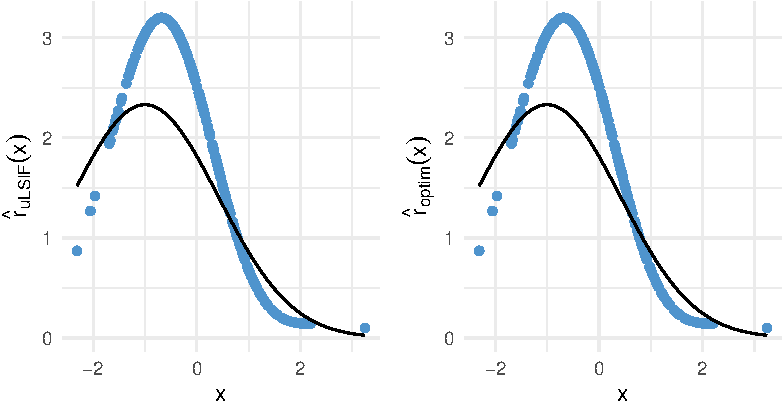
\includegraphics[keepaspectratio]{paper_files/figure-pdf/fig-AppA-1.pdf}}

}

\caption{\label{fig-AppA}Density ratio estimation using \texttt{ulsif()}
from the \texttt{densityratio}-package and using standard optimization
in \texttt{R}.}

\end{figure}%

\linespread{2}

If we were to perform cross-validation for hyperparameter selection, we
could run the \texttt{ulsif()}-function without specifying the
\texttt{sigma} and \texttt{lambda} arguments. The function then performs
a grid search over a predefined range of hyperparameters. Moreover, it
is possible to supply a vector of \texttt{sigma} and \texttt{lamdba}
values to \texttt{ulsif()}, after which cross-validation is
automatically performed.

\linespread{1}

\begin{Shaded}
\begin{Highlighting}[]
\NormalTok{fit }\OtherTok{\textless{}{-}} \FunctionTok{ulsif}\NormalTok{(x, y, }\AttributeTok{centers =}\NormalTok{ x, }\AttributeTok{scale =} \ConstantTok{NULL}\NormalTok{)}
\NormalTok{fit}
\end{Highlighting}
\end{Shaded}

\begin{verbatim}

Call:
ulsif(df_numerator = x, df_denominator = y, scale = NULL, centers = x)

Kernel Information:
  Kernel type: Gaussian with L2 norm distances
  Number of kernels: 250
  sigma: num [1:10] 0.0601 0.177 0.2971 0.4228 0.5583 ...

Regularization parameter (lambda): num [1:20] 1000 483.3 233.6 112.9 54.6 ...

Optimal sigma (loocv): 0.7045195
Optimal lambda (loocv): 1.43845
Optimal kernel weights (loocv): num [1:251] 0.03123 0.03174 0.02443 0.00876 0.01296 ...
 
\end{verbatim}

\linespread{2}

The model output shows the optimal \texttt{sigma} parameter out of a
vector containing ten values, and the optimal \texttt{lambda} parameter
out of a vector containing twenty values. The package also includes
density ratio estimation techniques, such as \texttt{kliep()},
\texttt{kmm()}, \texttt{spectral()}, \texttt{lhss()} and
\texttt{naive()}, that all work in a similar fashion. Additionally, the
package contains generic functions to \texttt{predict()} with,
\texttt{plot()}, or summarize (e.g., \texttt{summary()}) the fitted
models. Moreover, computationally intensive code is implemented in
\texttt{C++} through \texttt{Rcpp} (\citeproc{ref-Rcpp}{Eddelbuettel
2013}) and most functions allow for parallel computation through the
\texttt{openmp}-backend in \texttt{C++}. The interested reader is
referred to the package documentation
(\citeproc{ref-densityratio}{Volker 2023}) for additional information.

\section{\texorpdfstring{\(k\)-Nearest neighbor density ratio
estimation}{k-Nearest neighbor density ratio estimation}}\label{sec-app-B}

We note that density ratio estimation through \(k\)-nearest neighbor
density estimation can also be considered a direct approach to density
ratio estimation. Using \(k\)-nearest neighbors, an estimate of the
density can be obtained by \[
\hat{\pobs}(\bx_i) = \frac{k}{n-1} \cdot \frac{\Gamma(d/2 + 1)}{\pi^{d/2} B^d_k(\bx^{(\text{obs})}_i)},
\] where \(d\) denotes the dimensionality of the input data,
\(\Gamma(d/2 + 1) / \pi^{p/2}\) is a normalizing constant, and
\(B^d_k(\mathbf{x}^{(\text{obs})}_i)\) denotes the Euclidean distance of
each observation in \(\mathbf{x}^{(\text{obs})}\) to its \(k\)-th
nearest neighbor in \(\mathbf{x}^{(\text{obs})}\) raised to the power
\(d\) (see, e.g., \citeproc{ref-wang_divergence_2009}{Wang, Kulkarni,
and Verdu 2009};). Applying the same procedure for the denominator data
(i.e., the synthetic data), we can estimate the density ratio as \[
\begin{aligned}
\hat{r}(\bx_i) &= \frac{\hat{\pobs}(\bx_i)}{\hat{\psyn}(\bx_i)} \\
&= \frac{\frac{k}{n-1} \cdot \frac{\Gamma(d/2 + 1)}{\pi^{d/2} B^d_k(\mathbf{x}^{(\text{obs})}_i)}}{\frac{k}{m} \cdot \frac{\Gamma(d/2 + 1)}{\pi^{d/2} B^d_k(\mathbf{x}^{(\text{syn})}_i)}} \\
&= \frac{m}{n-1} \cdot \frac{B^d_k(\mathbf{x}^{(\text{syn})}_i)}{B^d_k(\mathbf{x}^{(\text{obs})}_i)},
\end{aligned}
\] where \(m\) denotes the number of observations in the synthetic data,
and \(B^d_k(\mathbf{x}^{(\text{syn})}_i)\) denotes the Euclidean
distance of each observation in \(\mathbf{x}^{(\text{obs})}\) to its
\(k\)-th nearest neighbor in \(\mathbf{x}^{(\text{syn})}\) raised to the
power \(d\). Accordingly, a direct estimate of the density ratio can be
obtained as \[
\hat{r}(\bx) = \text{diag}\{\tilde{B}^d_k(\mathbf{x}^{(\text{obs})})\}^{-1} \tilde{B}^d_k(\mathbf{x}^{(\text{syn})}),
\] where \(\tilde{B}^d_k(\mathbf{x}^{(\text{obs})})\) and
\(\tilde{B}^d_k(\mathbf{x}^{(\text{syn})})\) denote the vectors with
distances of each observation in \(\mathbf{x}^{(\text{obs})}\) to their
\(k\)-th nearest neighbor in \(\mathbf{x}^{(\text{obs})}\) and
\(\mathbf{x}^{(\text{syn})}\) raised to the power \(d\), multiplied by
the respective sample sizes.

Applying this estimate of the density ratio to the simulated data from
the univariate simulations, and setting \(k = 15 \approx \sqrt n\), as
suggested by the authors who introduced \(k\)-nearest neighbor density
estimation (\citeproc{ref-loftsgaarden_nonparametric_1965}{Loftsgaarden
and Quesenberry 1965}), we can compare the performance of the
\(k\)-nearest neighbor density ratio estimation to the density ratio
estimation through uLSIF.

\linespread{1}

\begin{figure}[t]

\centering{

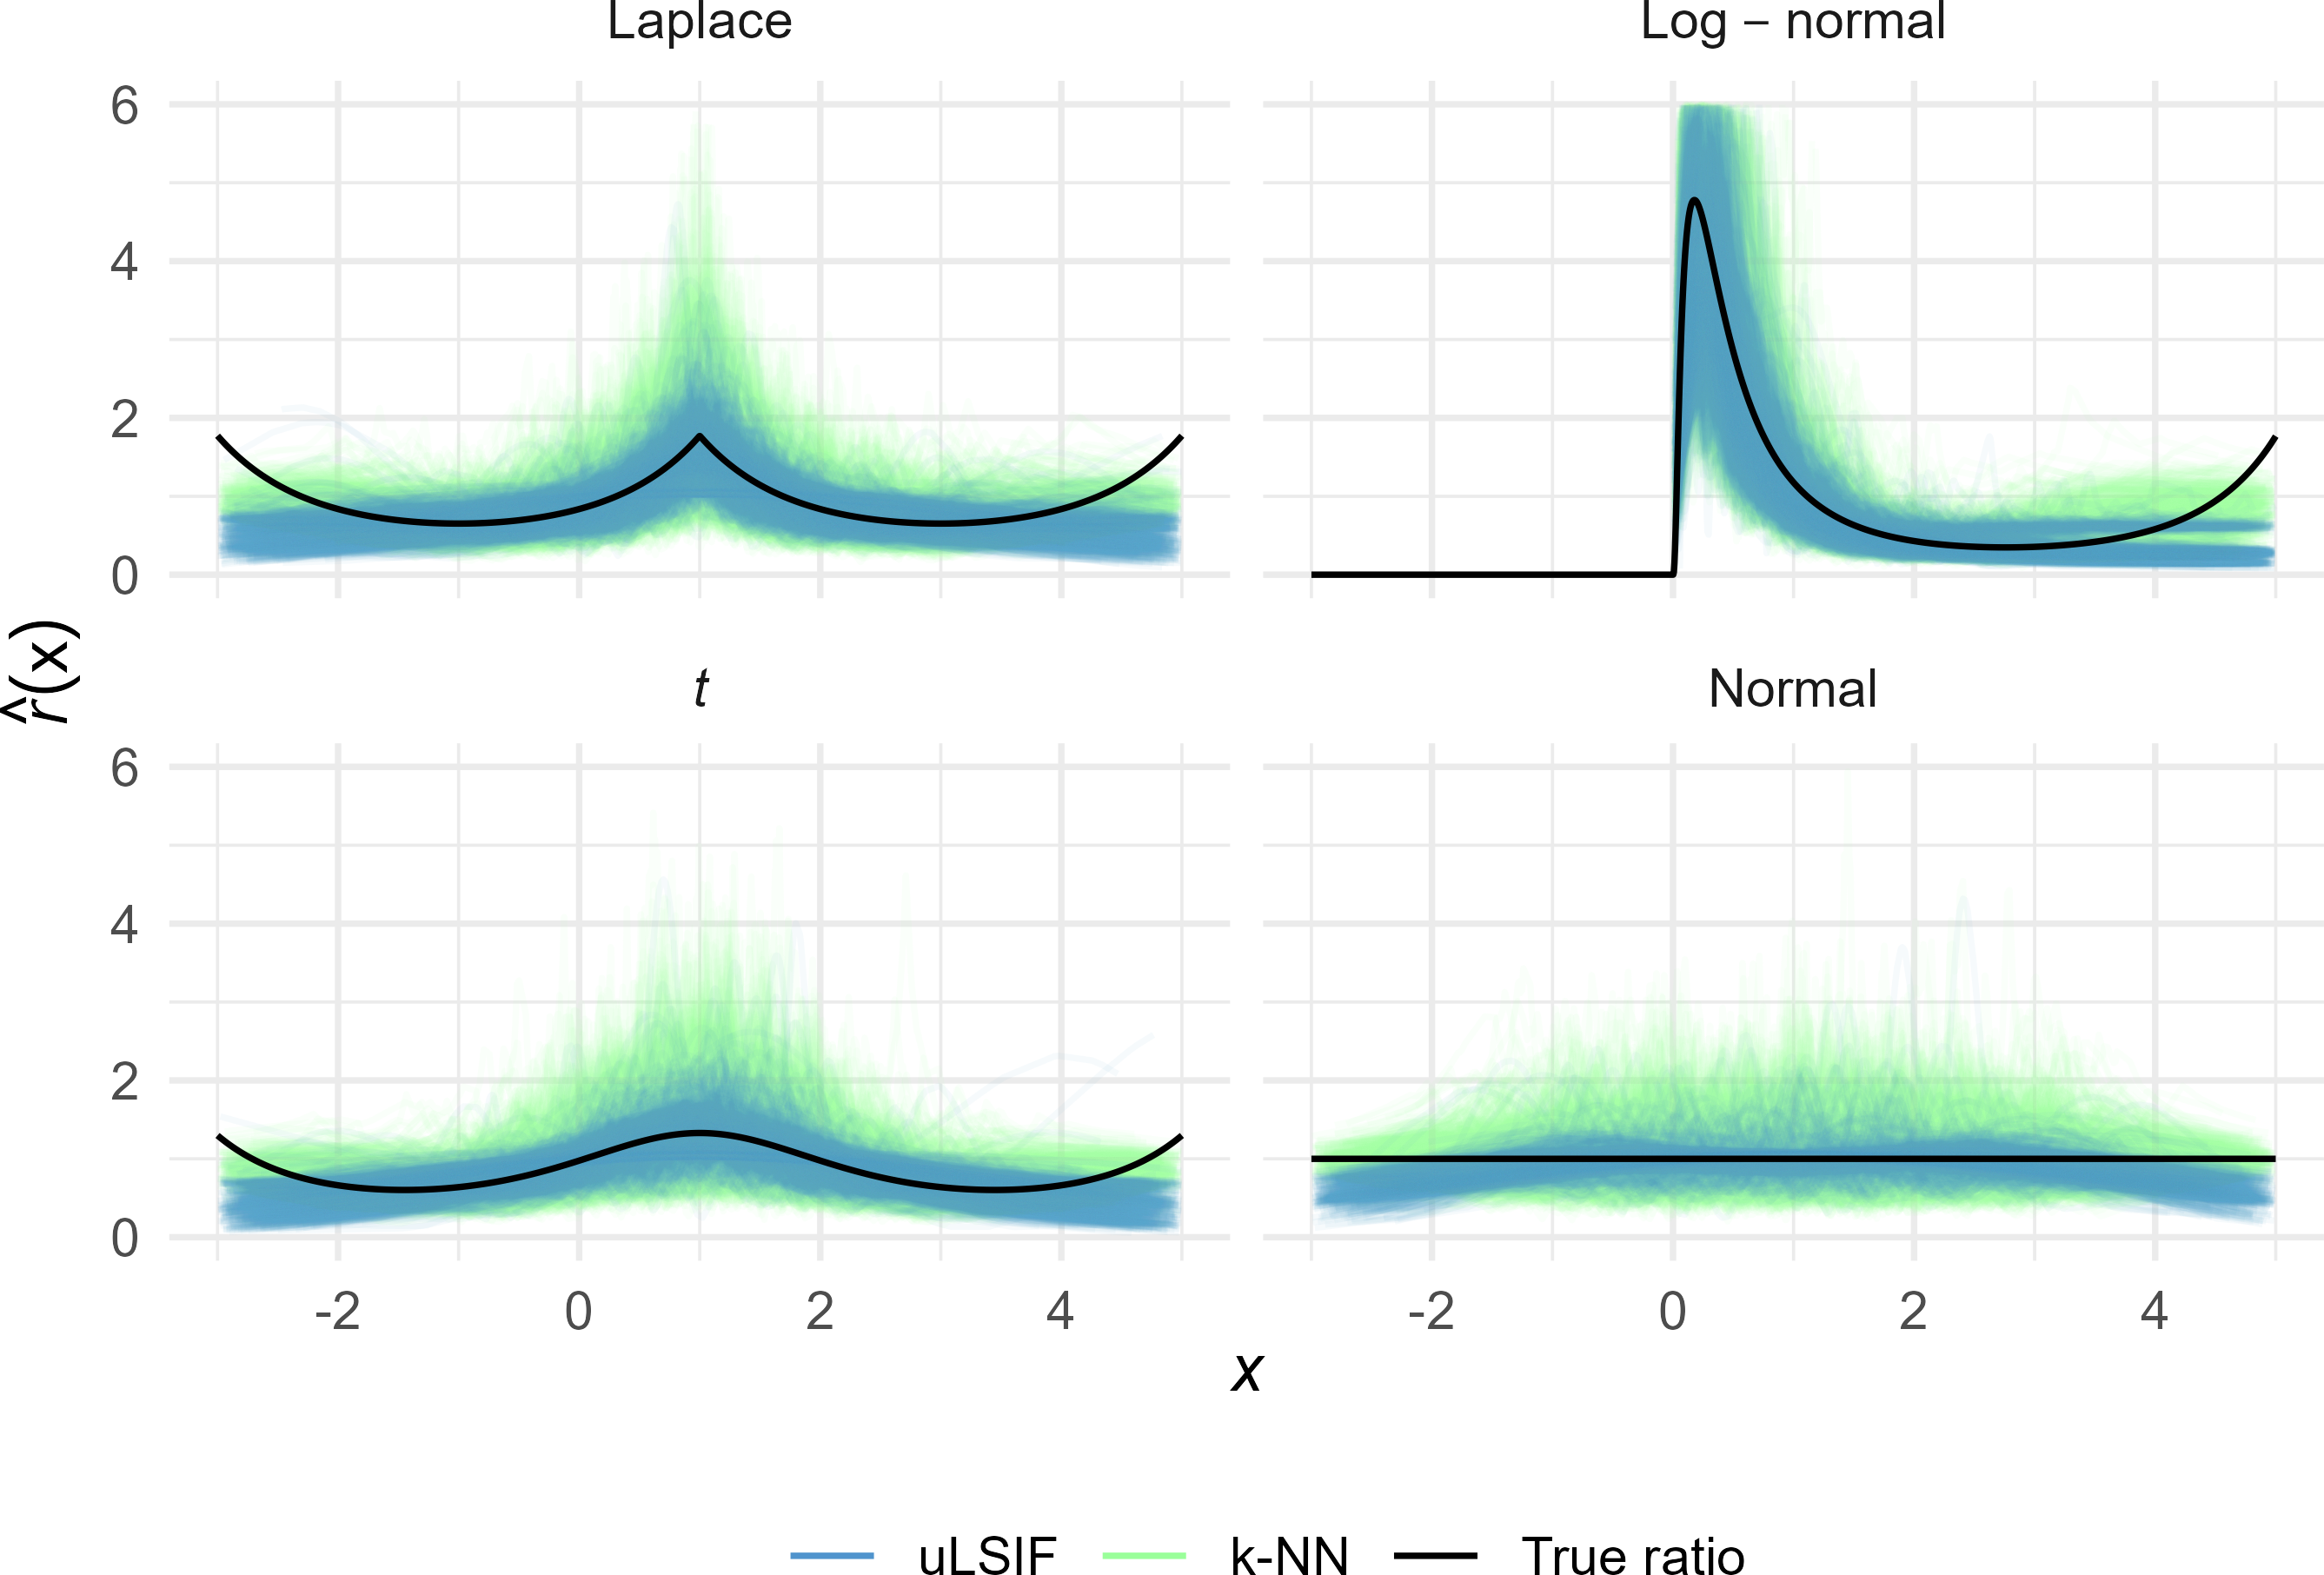
\includegraphics[width=1\linewidth,height=\textheight,keepaspectratio]{paper_files/figure-pdf/fig-AppB-1.png}

}

\caption{\label{fig-AppB}Density ratio estimation through \(k\)-nearest
neighbor density ratio estimation (\(k = 15\)) and uLSIF.}

\end{figure}%

\linespread{2}

It can be seen that the \(k\)-nearest neighbor density ratio estimation
performs well on average (the green lines in Figure~\ref{fig-AppB}),
especially in the center of the distribution. However, it suffers from a
similar bias in regions where the number of observations is low (as the
density ratio is typically underestimated in the tails). Moreover,
\(k\)-nearest neighbor density ratio estimation has much higher variance
than density ratio estimation through uLSIF, as can be seen by the fact
that the green lines cover a much wider band than the blue lines.




\end{document}
